\chapter{Physics: QFT crash course} 

The Standard Model (SM) of particle physics classifies all known
\index{particle!elementary}\index{Standard Model}
{\it elementary particles}, i.e. particles with no known substructure,
and describes three fundamental forces:\index{force!fundamental} the electromagnetic,
weak, and strong forces. Elementary particles can be divided into
\index{particle!matter}
{\it matter particles} (quarks and leptons); {\it gauge bosons}, which mediate
\index{boson!scalar}\index{boson!gauge}
the three aforementioned forces; and a {\it scalar boson}, the Higgs boson,
whose field interacts directly with elementary particles that thereby
acquire their mass. For each particle there exists a corresponding
antiparticle; sometimes a particle is its own antiparticle.
Figure~\ref{fig:SM} gives a schematic overview of the SM.

\begin{figure}
  \centering
  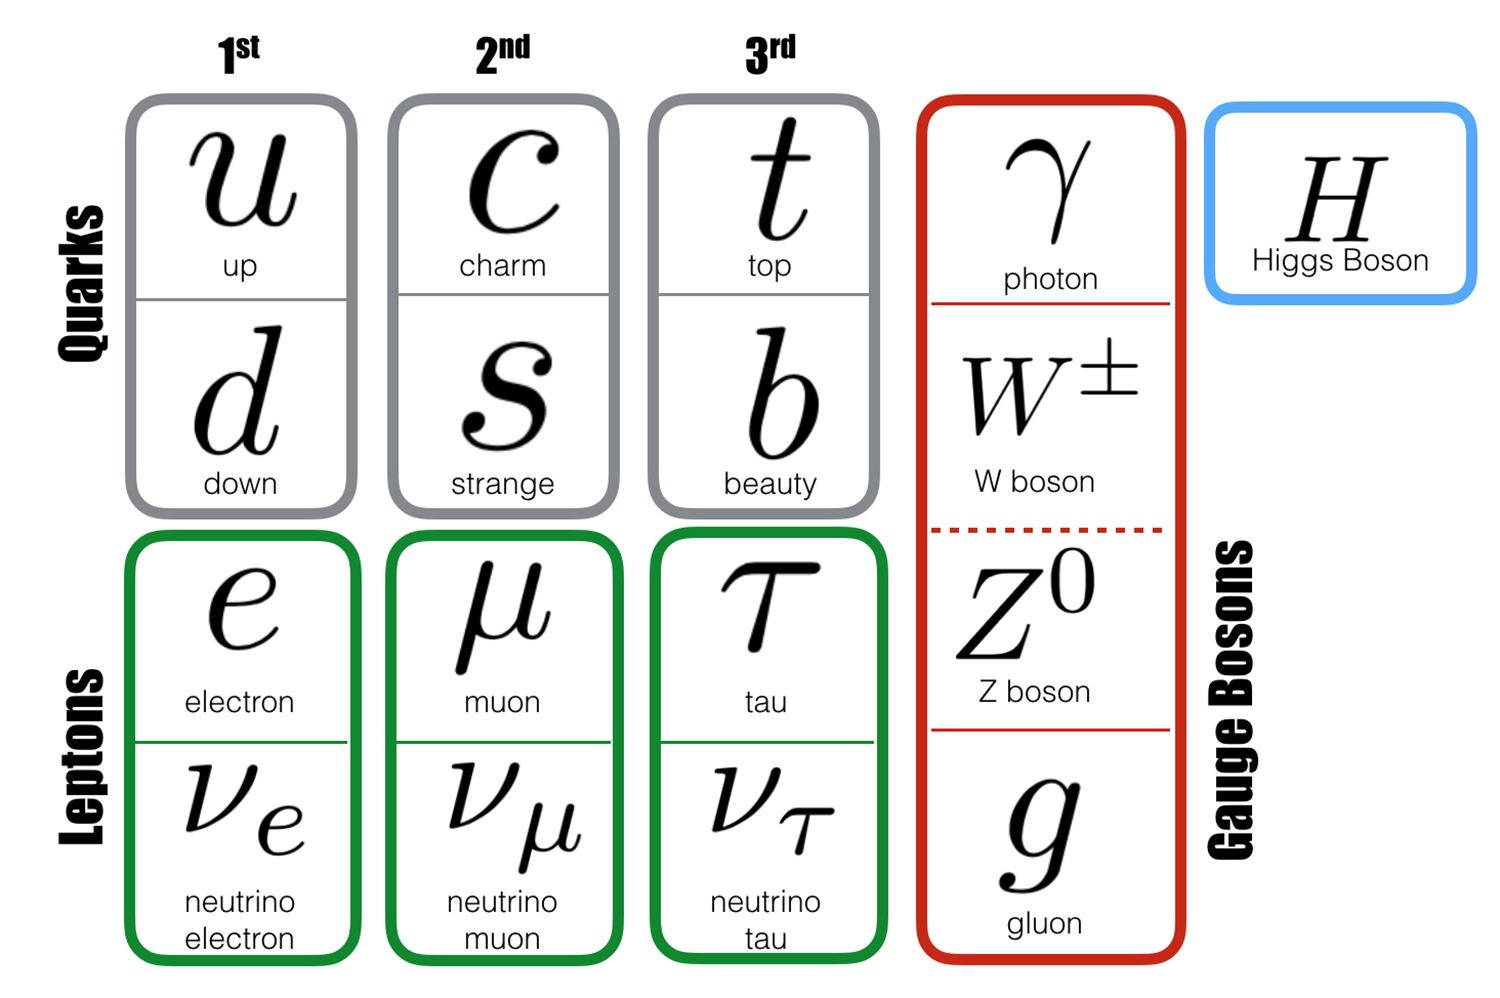
\includegraphics[width=0.80\linewidth]{figs/SM.png}
  \caption{Summary of elementary SM particles. The first three columns give
           the three generations of matter particles. Image taken
           from the Physics Institute at University of 
           Zurich~\cite{zurich_SM}.}
  \label{fig:SM}
\end{figure}

The theoretical framework underlying the SM is an example of a Quantum 
Field Theory (QFT). QFTs are consistent with both quantum mechanics and
relativity. Lattice gauge theories are a kind of QFT; therefore it is
important for the reader to know a little bit about them. A solid understanding
of QFT I think can only be achieved by taking courses along with a significant
amount of self study. In my case, that self study has required multiple years,
but you're a different person, so mileage may vary.

There are a lot
of different resources one can use to learn about QFT; for example when I was a
grad student I used Peskin and Schroeder~\cite{peskin_introduction_1995}
and Srednicki~\cite{srednicki_quantum_2007}. Far and away the most pedagogical
text book I've encountered is by Schwartz~\cite{schwartz_quantum_2014}, and it's
the one I recommend to newcomer in the field.
Nowadays there are also some very high quality lectures on YouTube,
for instance a series by Tong~\cite{tongQFT}, which I found had some other nice
introductory remarks. 
A timeline of particle discoveries can be found in
Ref.~\cite{wiki_particle_discoveries}. Another detailed historical overview
of the SM is given in Chapter 1 of Ref.~\cite{griffiths_introduction_2007}.

\section{An mnemonic history of the SM}

One could argue that the beginning of the SM history coincides with the
beginnings of modern particle physics. Since that depends on unifying
relativity, quantum mechanics, and field theory, one could arguably even take
Maxwell's equations as a starting point. 
There were also many interesting ideas that were not pursued or turned out
not to be correct yet still played some role in the history; I will not
discuss these. In some cases I may miss some discoveries that were also
important but less celebrated.

Given these ambiguities and the fact
that I am not at all a real historian, 
one might call what follows an ``approximate" history.
As I was writing this, I realized that I was trying to tell a story, i.e.
to write it in a way that one development would make sense or feel
motivated given a previous development. Usually that is a bit of an
oversimplification, but it helps me remember why certain discoveries were
significant, where some nomenclature comes from, and what it means. Hopefully it
also helps reveal how physicists think, how we are led to discoveries, and
ultimately why we believe our theories. So with these advantages in mind, I
rather decided to call it a ``mnemonic" history. 

Also while I was writing this, I learned a bunch of facts that I found
interesting but are probably a bit off-topic. Hence this mnemonic history is
densely packed with footnotes. For example I decided to start listing Nobel
prizes for some reason. By the time I realized doing this is tedious and does not
teach much, I somehow already felt pot-committed, so I ended up seeing this habit
through to the bitter end. 

\subsection{The fundamentals}

% pauli, jordan etc 1920s-30s how to quantize fields. 
% Failing to have theory with infinite num of dof,
% then tomonaga, schwinger, dyson, feynman. Can renormalize, QED discovered.
%   measurement of Lamb shift 1947. Bethe has explanation that gets refined
%   in QED, helps establish QFT.
% 1970s golden age: infinites understood through
% renormalization group wilson and kadanoff.

In 1897 J.J. Thomson did experiments with cathode rays\footnote{In a small
vacuum chamber with two electrodes, if a voltage is applied between them,
electrons will move between them. Televisions used to work by cathode ray tubes,
\index{cathode ray tube} where these electrons are deflected by magnetic fields
to make images on the screen.}
from which he concluded that electric charge must be carried by particles
with high charge-to-mass ratio, the electrons\footnote{He received the 1906
Nobel in physics for this work.} 
To explain why atoms are overall electrically neutral, Thomson guessed that
electrons are distributed in a sea of positive charge, which is the
well known {\it plum pudding model}.\index{plum pudding model} This was
disproved by Rutherford in his famous gold foil
experiment~\cite{rutherford_scattering_1911}, in which he discovered
the atomic nucleus. Shortly thereafter, he discovered the
proton~\cite{rutherford_collision_1919}.
Bohr proposed his model~\cite{bohr_constitution_1913}
of hydrogen, supposing it to be made of a proton and an electron, which agreed
well with experiment\footnote{He got the 1922 Nobel for his
contributions understanding atomic structure.}. Extending this theory to 
heavier elements by supposing
they are also made of only protons and neutrons however fails, since e.g. helium
is four times as heavy as hydrogen. This difficulty would not be sorted out
until the early 1930s, when Chadwick discovered~\cite{chadwick_possible_1932}
the neutron\footnote{1935 Nobel for him.}.


These early discoveries successfully explained many details of the atom; however
the fact that atomic nuclei are made of particles with only positive or zero
electric charge still required explanation.
Hence for some time, physicists
knew there must be some {\it strong force}\index{force!strong} that opposes
Coulomb repulsion and binds nucleons into nuclei.
Such particles held together by strong interactions are called
{\it hadrons}.\index{hadron} Nowadays we also use the terms {\it meson}
\index{meson} and {\it baryon}\index{baryon} to refer to hadrons made of
two quarks and three quarks, respectively\footnote{This naming scheme
comes from particle weights. At the time, known leptons were light, 
baryons were heavy, and mesons were somewhere in the middle. In retrospect it
would have been nicer to name them something like $n$-hadrons, but alas it would
take several decades for us to see that hadrons are made of quarks.}.


One of the earliest, important discoveries of the quantized natures of particle
properties is the celebrated Stern-Gerlach
experiment~\cite{gerlach_experimentelle_1922a,gerlach_magnetische_1922b,gerlach_experimentelle_1922c}. 
In this experiment, silver atoms
are deflected by an inhomogeneous magnetic field.
Besides having demonstrated that particles have intrinsic spin, it showed that
the spin is quantized and that measurements of spins along perpendicular axes
``reset" the spin state, and it provided the first measurement of the electron
magnetic moment.


Around this time, physicists were also beginning to see the particle nature of
light. In particular, Planck proposed~\cite{Planck:1901tja} 
that light may come in discrete packets of
energy in order to avoid the \index{ultraviolet catastrophe}ultraviolet 
catastrophe\footnote{1918 Nobel.}.
Einstein took this proposal seriously~\cite{Einstein:1905cc}, 
and used it to explain the photoelectric
effect\footnote{1922 Nobel for him. Also in 1905 he published his first
papers on special relativity, as well as a paper on Brownian motion.}. 
A careful study~\cite{millikan_direct_1916} of the photoelectric effect by 
Millikan showed that
Einstein's interpretation explained the photoelectric effect well\footnote{He
got the 1923 Nobel in part for this reason.}. Finally
Compton showed\footnote{He shared the 1927 Nobel for this.} 
that light scattered from a particle shifts by the Compton
wavelength\index{wavelength!Compton}
\begin{equation}
  \lambda_c=\frac{\hbar}{2mc},
\end{equation}
where $m$ is the target particle's mass, which one can derive by assuming light
is made of particles with zero rest mass~\cite{Compton:1923zz}.
Altogether these discoveries convinced physicists light behaves as a particle
at short enough length scales, which is the usual photon.\index{photon}


If light is to be quantized, it requires a theory that knows about both quantum
mechanics and special relativity, i.e. it needs QFT. 
The standard line of thinking can be cast in this way: One starts with
the Schr\"odinger 
equation~\cite{Schrodinger:1926gei,Schrodinger:1926vbi,Schrodinger:1926qnk,Schrodinger:1926xyk}
for a spinless, non-relativistic particle
of mass $m$ in the position basis,
\index{Schr\"odinger equation}
\begin{equation}
i\hbar\partial_t\psi=-\frac{\hbar^2}{2m}\nabla^2\psi.
\end{equation}
If we instead use a relativistic Hamiltonian and square the differential
operators on each side, we get the 
{\it Klein-Gordon equation}~\cite{Klein:1926tv,gordon_comptoneffekt_1926}
\index{Klein-Gordon equation}
\begin{equation}
-\hbar^2\partial_t^2\psi=\left(-\hbar^2c^2\nabla^2+m^2c^4\right)\psi.
\end{equation} 
While this is at least relativistically sensible, one can show that this
squaring of operators
leads to state normalization being time-dependent, i.e. probability is not
conserved. The situation was finally rescued by Dirac\footnote{Dirac
and Schr\"odinger shared the 1933 Nobel.}, who realized that
one could have a relativistically sensible equation that is first-order
in its operators by introducing some matrices and a spin component
to the wavefunction~\cite{Dirac:1928hu,Dirac:1928ej}. The result is the 
{\it Dirac equation}\index{Dirac equation}
\begin{equation}
i\hbar\slashed{\partial}\psi=mc\psi.
\end{equation}

The corresponding Hamiltonian for the Dirac equation is traceless, which
tells you that the energy eigenvalues cancel out, i.e. 
it suggests there are states of
negative energy. These negative energy states indicate that the theory
has no ground state. In order to prevent this infinite cascade into increasingly
negative energies, he speculated that these infinitely many states are already
occupied, which is referred to as \index{Dirac sea}the {\it Dirac sea}; 
the Pauli exclusion principle then prevents this infinite descent. 
If an electron in the sea were excited, it would leave behind a vacancy
that would manifest itself as a positively charged particle. This was the
prediction of the existence of the \index{positron}positron, which
was discovered\footnote{1936 Nobel.} in 1932 by Anderson~\cite{Anderson:1933mb}.
Later St\"uckelberg~\cite{Stueckelberg:1941rg} and
Feynman~\cite{feynman_theory_1949} would introduce the modern interpretation
of the positron: rather than being a hole left in the Dirac sea,
the previously negative energy states are to be understood as the
positive energy states of a different particle.


One of the last kinds of fermions needed to complete our particle collection
are the neutrinos. Before 1930, there was a problem with $\beta$-decay
\index{decay!beta} 
which is any decay emitting an $e^+$ or $e^-$ from
an atomic nucleus: Energy was not conserved. In particular if one assumes
a general $\beta$-decay process functions like
\begin{equation}
  A\to B+e^-,
\end{equation}
one can use conservation of four-momentum to find the electron energy.
The measured energy was found to fluctuate and be smaller than what four-momentum
conservation delivers. Pauli
suggested\footnote{Rather than being documented in a publication, this seems to
come from a letter written by Pauli addressed to a conference in T\"ubingen.
It opens, ``Liebe Radioaktive Damen und Herren".} that this missing energy
lies with an as-yet-undetected, weakly interacting particle, the
electron neutrino. The electron neutrino would not be 
discovered\footnote{1995 Nobel.}\index{neutrino!electron}
until the mid 1950s by Cowan and Reines~\cite{Cowan:1956rrn}.

\subsection{Weak and strong forces}

\index{interaction!weak}
In the early 1930s, Fermi published\footnote{Apparently he originally attempted
to publish it in {\it Nature}, but they rejected it because
it because ``it contained speculations too remote from reality to be of interest
to the reader".} his theory of the 
\index{decay!beta}$\beta$-decay~\cite{fermi_tentativo_1934}
\begin{equation}
  n\to\text{p}+e^-+\bar{\nu}_e.
\end{equation}
He introduced an effective 4-point interaction directly linking the four
particles in the above process.
Shortly thereafter, Yukawa~\cite{yukawa_interaction_1935} put forward that this
interaction should include another field with corresponding quantum that
mediates this interaction\footnote{Nowadays we designate as
{\it Yukawa interaction} any interaction between
Dirac fields and scalar fields of the form\index{interaction!Yukawa}
$g\bar{\psi}\phi\psi$ or $g\bar{\psi}i\gamma_5\phi\psi$.}, 
sort of like how the photon mediates the
electromagnetic interaction. Another salient point of this paper is
the introduction of the {\it Yukawa potential}\index{potential!Yukawa}
giving the potential of a gauge boson of mass $m$:
\begin{equation}
  V(r)=-g^2\frac{e^{-\alpha m r}}{r}.
\end{equation}
Here $g$ is the gauge coupling and $r$ is the interaction range. One sees that
massless gauge bosons have a Coulomb-like potential, while massive ones
are suppressed exponentially\footnote{One can also show that the Fourier
transform of this potential is the propagator, which we will discuss later.},
which gives an explanation why the weak force has a short interaction range. 
Besides already hinting massive weak bosons, this paper is considered to be
one of the first theories of the strong force; from this perspective the
proton and neutron exchange massive mesons, which therefore have a limited
interaction range\footnote{1949 Nobel.}.

\begin{figure}
  \centering
  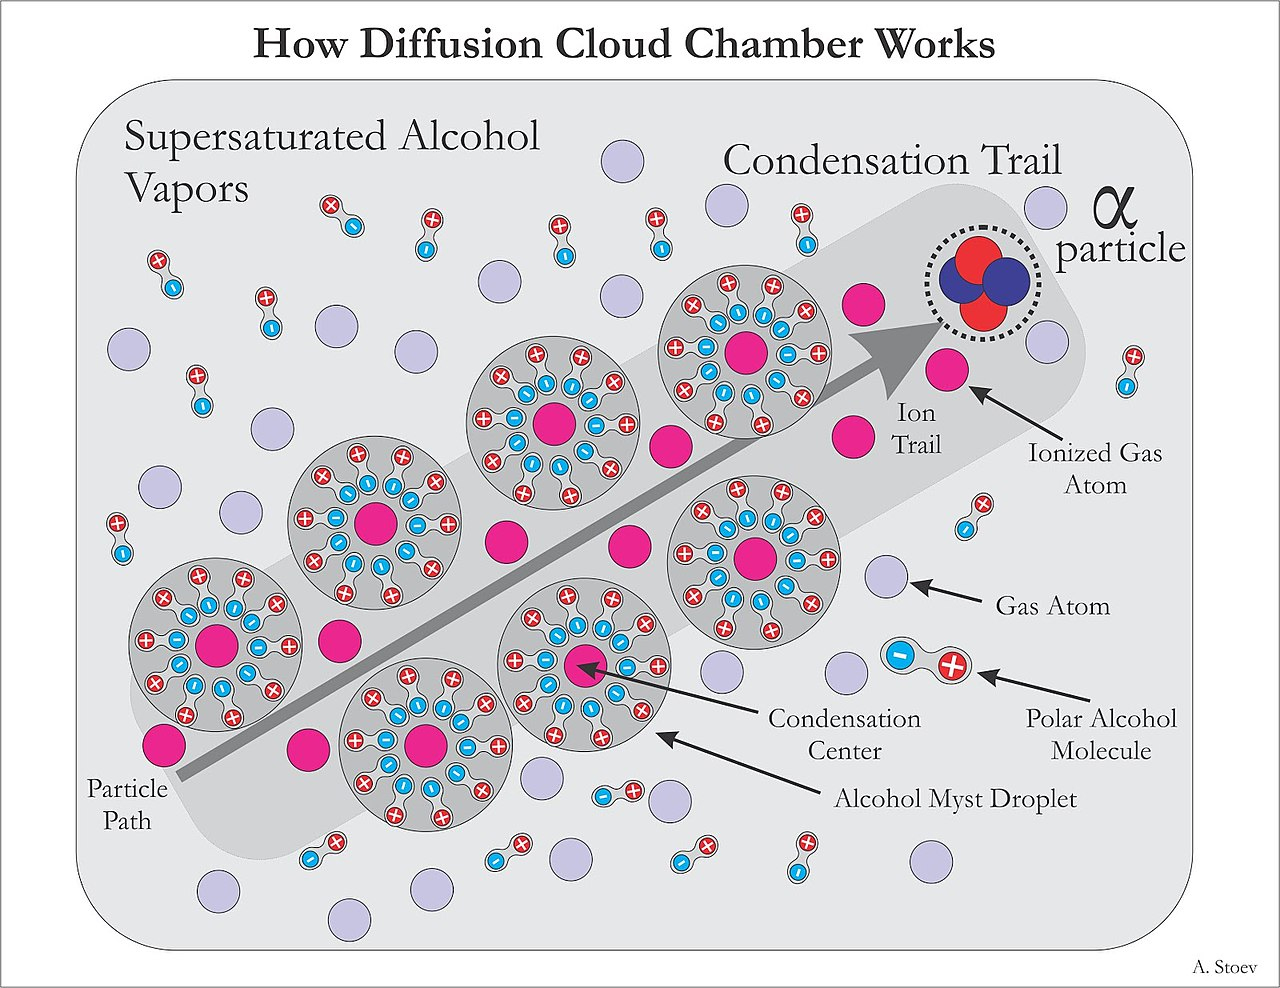
\includegraphics[width=\linewidth]{figs/Diffusion_Cloud_chamber_explained.jpg}
  \caption{Cloud chambers consist of a sealed environment with some vapor
           of e.g. alcohol. As a charged particle moves through the vapor, it knocks
           electrons off the gas; the resulting ions attract the polar molecules,
           which leaves a visible trail for a short time. To identify particles,
           you can see e.g. if they were deflected. C. T. R. Wilson is generally 
           credited as the inventor of cloud chambers, and he shared the 1927 Nobel
           in physics for it. They were extremely popular to use in experiment
           for finding particles until the later invention of the bubble chamber.
           Image taken from Wikipedia~\cite{wiki_cloud}.}
  \label{fig:cloud}
\end{figure}

An early experimental search of cosmic ray\footnote{A {\it cosmic ray} is a high
energy proton or atomic nucleus that originates somewhere from space. They were
discovered in the early 1910s by Hess, which got him the 1936 Nobel.}
\index{cosmic ray} measurements using
cloud\index{cloud chamber} chambers (see \figref{fig:cloud}) 
found the muon~\cite{neddermeyer_note_1937}, which was originally 
mistaken\footnote{Indeed the muon and pion masses are pretty close to each
other, sitting at about 106~MeV and 140~MeV, respectively.}
as the meson that Yukawa suggested. An experiment in the late 1940s showed that
the muon does not interact very strongly with atomic
nuclei~\cite{conversi_disintegration_1947}, which rules it out as the strong
force mediator. Thankfully for Yukawa the
pion\footnote{Pions\index{pion}\index{meson!pi@$\pi$} are the lightest
mesons. They are made of pairs of up and down quarks.} was
discovered~\cite{lattes_processes_1947} in 1947\footnote{And got Powell
the 1950 Nobel for it. It is actually a bit puzzling that he is the only
recipient of this prize, most obviously because only three other scientists were
on his team. Furthermore this prize credits him for his ``development of
photographic method for studying nuclear processes", even though this method was
pioneered by other physicists such as Blau and Wambacher.}.


\index{interaction!strong}
In the late 1940s and early 1950s, the {\it kaon} ($K$)~\cite{rochester_evidence_1947}
\index{meson!K@$K$} and {\it lambda} ($\Lambda$)~\cite{hopper_evidence_1950}
\index{baryon!l@$\Lambda$} hadrons were discovered. A kaon
consists of light quark and a strange, while a lambda baryon binds two light
quarks with one from a higher generation. {\it Strangeness}\footnote{We now 
\index{strangeness}
identify strangeness $S$ as
$$
  S\equiv\#\,\text{anti-strange quarks}-\#\,\text{strange quarks}.
$$}
was originally proposed as a conserved quantity to explain the relatively long
lifetimes of these particles~\cite{pais_remarks_1952,gell-mann_isotopic_1953,
pais_baryon-meson-photon_1953,tadao_charge_1953}.
Ne'eman~\cite{neeman_derivation_1961},
Gell-Mann~\cite{gell-mann_symmetries_1962}, and
Zweig~\cite{zweig_su3_1964} proposed\footnote{Gell-Mann would receive the 1969
Nobel for his contributions to understanding elementary particle
classification.} that these hadrons could be classified
according to the irreducible representations of $\SU(3)$, a viewpoint which
Gell-Mann called the \index{eightfold way}{\it eightfold way}\footnote{This
name is inspired by the eightfold path of Buddhism.}, examples of which are
illustrated graphically in \figref{fig:eightfold}. Gell-Mann
referred to the fundamental units as {\it quarks}\footnote{Gell-Mann borrows
this name from an excerpt of James Joyce's {\it Finnegan's Wake} that begins
``Three quarks for Muster Mark".
Gell-Mann was a bit of a fanciful guy I guess.}.
At first it was not clear that this quark viewpoint was more than a
purely mathematical construction, however deep inelastic
scattering\index{scattering!deep inelastic}
experiments at the Stanford Linear Accelerator (SLAC) showed that
protons are made of smaller particles, and are therefore not
elementary~\cite{bloom_high-energy_1969,breidenbach_observed_1969}.
This alone did not convince the community that quarks were 
real\footnote{For a while it was fashionable to refer to rather refer to
nucleon constituents as {\it partons}\index{parton}, a term coined
by Feynman.}, but
subsequent discoveries would solidify the quark model,
for example the 1964 discovery\cite{barnes_observation_1964} 
of the\index{baryon!$\Omega$} 
$\Omega$ baryon\footnote{An $\Omega$ baryon is any baryon not
containing $u$ or $d$ quarks. The $\Omega$ with a $t$ is not expected
to exist in the SM because the $t$ lifetime is too short to
interact strongly. The title of the discovery paper refers 
to\index{hyperon} {\it hyperons}, which are any baryons with
at least one $s$ quark. Hence $\Omega$ baryons are a type of hyperon.}.

\begin{figure}[t]
  \centering
  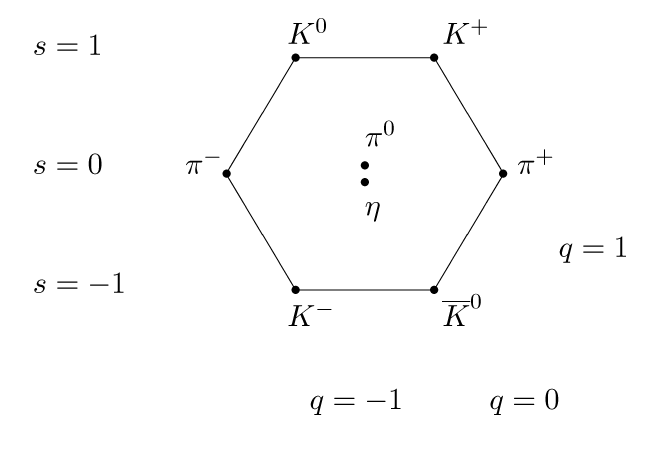
\includegraphics[width=0.48\linewidth]{figs/Meson_octet.png}
  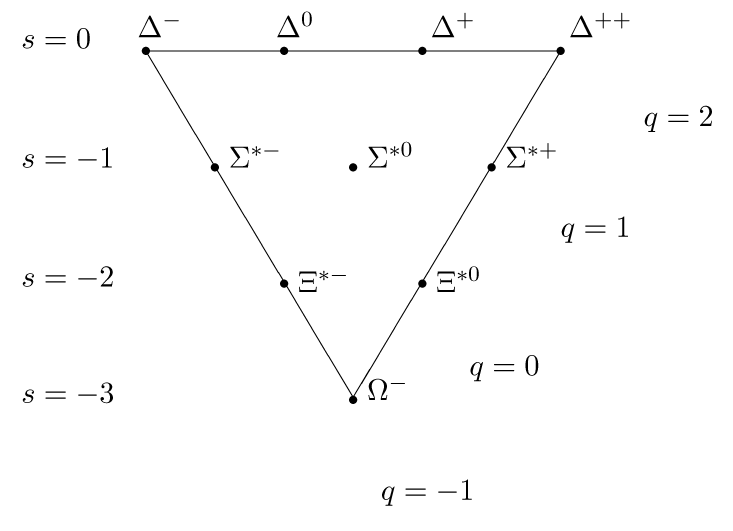
\includegraphics[width=0.48\linewidth]{figs/Baryon_decuplet.png}
  \caption{{\it Left}: Spin-0 pseudoscalar meson octet. (See
           \tabref{tab:discreteSymm} for a definition of
           pseudoscalar.) {\it Right}:
           Spin-3/2 baryon decuplet. The $s$ represents strangeness,
           with all particles in the same horizontal row having the
           same strangeness. Electric charge is represented by $q$,
           with all particles along the diagonal having the same
           electric charge. Images taken from
           Wikipedia~\cite{wiki_eightfold}.}
  \label{fig:eightfold}
\end{figure}

From here it was shown possible to formulate a QFT for the strong interaction
based on $\SU(3)$~\cite{fritzsch_advantages_1973}, which we
call quantum chromodynamics (QCD).\index{quantum chromodynamics}
The mediators are called
{\it gluons}\index{gluon} with the adjoint representation delivering
eight possible color combinations.
Gross, Wilczek~\cite{gross_d.j._ultraviolet_1973} and
Politzer~\cite{politzer_reliable_1973} demonstrated
{\it asymptotic freedom}\footnote{They got the 2004 Nobel for this.}
\index{asymptotic freedom} in this QFT, i.e. they showed that the
strong coupling decreases with increasing interaction strength, which is
consistent with the fact that one does not observe free quarks\footnote{At
least not at typical temperatures and densities.}.
This theoretical observation is buttressed by strong coupling
expansions in the lattice formulation, introduced by 
Wilson~\cite{wilson_confinement_1974}, which show that the potential
energy between two infinitely heavy quarks grows linearly with
increasing separation
(see \secref{sec:hqfe}).
%creutz_monte_1980
%wilson_RG 1 and 2

We round out this section with a short timeline of discoveries of the
remaining QCD particles. In 1974 the discovery of the
$J/\Psi$-meson\index{psion} or {\it psion}\footnote{The $J/\Psi$ consists
of a $\bar{c}c$ pair. This is also sometimes called {\it charmonium}.
\index{charmonium}} at both Brookhaven National Lab (BNL) and
SLAC~\cite{augustin_discovery_1974,aubert_experimental_1974} demonstrated
the existence of the charm quark\footnote{Richter and Ting got the 1974
Nobel prize in physics for this.}, adding further evidence to
the validity of the quark model. The $J/\Psi$ discovery marks the beginning of a
period of rapid discoveries in particle physics sometimes referred to as the
``November Revolution".\index{November Revolution} The existence of the bottom
quark was demonstrated in 1977 at Fermilab~\cite{herb_observation_1977} when the
$Y$-meson\footnote{A $Y$-meson\index{meson!Y} is a $\bar{b}b$ bound state. This is
sometimes called \index{bottomonium}{\it bottomonium}.} was discovered.
In 1979 we found experimental evidence for the
gluon via indirect observations~\cite{barber_discovery_1979} at the
Deutsches Elektronen-Synchrotron (DESY). In part because it is the
heaviest quark, the top quark would not be discovered until
1995~\cite{abachi_observation_1995,abe_observation_1995}
at Fermilab.


\subsection{Unification}


In the mid 1950s, Lee and Yang~\cite{lee_question_1956} suggested possible
experimental tests to search for parity violation in weak interaction 
processes\footnote{Lee and Yang won the 1957 Nobel prize for this.}.
Shortly thereafter, Wu et al.~\cite{wu_experimental_1957} demonstrated parity
violation in the $\beta$-decay of \ce{^{60}Co},
a result which was verified by Garwin et al.~\cite{garwin_observations_1957}. 
The theory of the weak interaction was extended by Gell-Mann and
Feynman~\cite{feynman_theory_1958} to accommodate parity violation by
introducing vector-axial currents.
That $\beta$-decay proceeds through vector-axial currents was
experimentally verified shortly thereafter~\cite{goldhaber_helicity_1958}.


The unification of the weak and electromagnetic forces began already with
Glashow in 1961~\cite{glashow_partial-symmetries_1961}, where
he puts forward the $\SU(2)\times \U(1)$ symmetry group. 
Still, this theory was not known to be renormalizable.
Also the weak interaction is short range, but this suggests that the mediating boson 
should be massive according to Yukawa. On the other hand, 
massive gauge bosons superficially spoil gauge invariance.


In superconductivity, Ginzburg-Landau theory~\cite{ginzburg_theory_1950}
gives solutions with effective mass. Nambu applied\footnote{2008 Nobel prize.} 
this to particle
physics~\cite{nambu_axial_1960,nambu_dynamical_1961,nambu_dynamical_1961-1},
but this implied the existence of Goldstone modes that are not observed.
Higgs~\cite{higgs_broken_1964} and Brout and Englert~\cite{englert_broken_1964}
noticed\footnote{Higgs and Englert received the 2013 Nobel for this.} 
that by strategically choosing 
the gauge, one can simultaneously
eliminate the Goldstone modes, add a mass term to gauge bosons, and a scalar
boson, the Higgs boson.\index{Higgs!boson}
We will discuss spontaneous symmetry breaking and Goldstone's theorem
\index{spontaneous symmetry breaking} in \secref{sec:ssb}. The Higgs
mechanism is discussed in detail in \apref{ap:spec_higgs}.


The original Higgs-Brout-Englert mechanism was demonstrated only for massive
QED; Kibble extended this idea to non-abelian
groups~\cite{kibble_symmetry_1967}. Weinberg~\cite{weinberg_model_1967}
and Salam~\cite{salam_weak_1968} applied Kibble's results to Glashow's
$\SU(2)\times\U(1)$ idea\footnote{And shared the 1979 Nobel for it.}. 
They demonstrated that one can generate masses
for weak gauge bosons along with electrons and muons, while still leaving
neutrinos massless. This approach also predicted neutral weak currents,
which were discovered shortly thereafter by the Gargamelle
experiment~\cite{hasert_observation_1974}. The $W$ and $Z$ bosons would
be discovered at the European Organization for Nuclear Research (CERN)
in the early 1980s~\cite{aubert_ratio_1983,arnison_experimental_1983}.


In 1963, Cabibbo introduced the {\it Cabibbo angle}\index{Cabibbo angle} allowing
for quark mixing in weak interactions~\cite{cabibbo_unitary_1963} to
explain the lifetimes of heavier hadrons. The suppression of flavor changing
neutral currents was explained in the early 1970s through the GIM\index{GIM mechanism}
mechanism~\cite{glashow_weak_1970}, but in order for this mechanism to work,
one needed full doublets of quarks and leptons.
Then Kobayashi and Maskawa predicted the existence of a third
generation~\cite{kobayashi_cp_1973}, since three quark generations are the
minimal amount needed to allow CP violation in the quark sector\footnote{They
shared the 2008 Nobel along with Nambu.}. The full quark mixing matrix
is known as the CKM matrix.\index{CKM matrix} Neutrino mixing is also handled
through a mixing matrix, the so-called PMNS matrix.\index{PMNS matrix} 
We discuss neutrino mixing in detail
in \apref{ap:spec_neutrino}.


In the early 1970s, t'Hooft and Veltman
showed\footnote{1999 Nobel prize for them.} these theories are
renormalizable~\cite{t_hooft_regularization_1972}. Together the Higgs mechanism
and renormalizability of the SM allow one to consistently generate gauge boson
masses while ensuring its applicability at all energy scales.
Furthermore CERN's 2012 discovery of the Higgs 
boson~\cite{aad_observation_2012,chatrchyan_observation_2012} shows that Higgs mechanism
corresponds to reality, rather than being just a mathematical trick to 
consistently approach massive elementary particles.



\section{Introductory remarks about QFT} 

Here I just want to list some things that seem to be true about the universe,
and therefore our underlying theory should reflect these things. For example:
\begin{enumerate}
  \item Causal influences seem to be {\it local}, i.e. there is no
        action-at-a-distance.
  \item Elementary particles are completely and perfectly indistinguishable.
\end{enumerate}
One way to make sense of these two points is to assume the existence of 
{\it fields},\index{field} math objects whose pre-image is all space-time.
That the field value depends on its space-time coordinate allows it to be local,
and all elementary particles are viewed as excitations of the field. Since all
particles are excitations of the same object, it is therefore unsurprising that
they would be indistinguishable.

Related to point (1) above, and as already mentioned in the introduction, we
would like our theories to have this property:
\begin{enumerate}
  \setcounter{enumi}{2}
  \item QFT should be consistent with special relativity.
\end{enumerate}
Demand (3) leads in part to the Klein-Gordon and Dirac equations, and from these
we will find that particle number is not conserved.
A fundamental QFT length scale can be heuristically derived from this statement 
as follows: Consider an elementary particle in a box of length $L$. By the 
uncertainty principle, we have
\begin{equation}
  \Delta p\gtrsim \hbar/2L,
\end{equation}
which means according to relativity,
\begin{equation}
  \Delta E\gtrsim \hbar c/2L.
\end{equation}
If the energy uncertainty is large enough, i.e. large enough to support a
particle-antiparticle pair, we conclude
\begin{equation}
  \Delta E\approx 2mc^2 \gtrsim\hbar c/2L.
\end{equation}
We then introduce the Compton wavelength\footnote{I guess if
one uses $\hbar$ instead of $h$ this is rather the {\it reduced} Compton
wavelength. But I somehow always work using $\hbar$ instead of $h$, so I opted
to abuse this convention a little.}\index{wavelength!Compton}
$\lambda_c=\hbar/mc$. This argument delivers an interpretation for 
$\lambda_c$:
\begin{equation}
  L \gtrsim \lambda_c/4
\end{equation}
is a distance threshold\footnote{I have also seen $\lambda_c/2$ as the threshold,
which comes when you think the energy uncertainty only has to be large enough to
support a single particle. But in QFT particles are always created from the
vacuum in particle-antiparticle pairs due to conservation laws.} below which 
you have to worry about QFT. Below this scale, you are likely to detect
particle-antiparticle pairs of the species you are examining, which you cannot
distinguish, and it becomes difficult to speak a unique particle at all. In that
sense the Compton wavelength gives a characteristic length scale for a
particle. One can compare this with the particle's de Broglie wavelength
\index{wavelength!de Broglie}$\lambda_v=\hbar/mv$, where it behaves in a well-defined way as a wave.


%\section{The principle of stationary action}
%This section follows a fairly well known and delightful lecture by Feynman
%\cite{caltech}.

\index{limit!classical}\index{non-relativistic limit}
\section{The non-relativistic and classical limits}

In this section I briefly give some intuition for how mundane Newtonian
physics can be recovered from the more esoteric relativistic and quantum
theories. Namely \index{limit!non-relativistic} I want to focus on 
the following two phrases:
\begin{enumerate}
  \item The non-relativistic limit is $c\to\infty$.
  \item The classical limit is $\hbar\to0$.
\end{enumerate}
I do not think I have the understanding to prove anything, but at least I
can provide some ideas and examples that can make you believe these
two statements.

The non-relativistic limit is, I think, the easier to understand. When we
learn about relativity, the speed of light $c$ is taken as a ``cosmic speed
limit"; correspondingly, sending $c\to\infty$ lifts the speed limit, and
so perhaps it's not surprising that Galilean physics is recovered.
More explicitly, we can see what happens to the Lorentz factor $\gamma$ and
Einstein velocity addition formula under these limits. For the former
we find
\begin{equation}
  \lim_{c\to\infty}\gamma
  =\lim_{c\to\infty}\frac{1}{\sqrt{1-v^2/c^2}}=1,
\end{equation}
i.e. there is no longer any time dilation or length contraction.
Meanwhile when $c\gg v$, we find for the velocity addition formula 
\begin{equation}
  v_1\oplus v_2
  =\frac{v_1/c + v_2/c}{1+v_1v_2/c^2}
  \approx \frac{v_1}{c} + \frac{v_2}{c}, 
\end{equation}
i.e. it reduces to Galilean velocity addition.

For the classical limit, one can look at specific, simple examples, such as
the quantum harmonic oscillator. In QM, the energy levels of this system
are given by
\begin{equation}
  E_n=\hbar\omega\left(n+\frac{1}{2}\right).
\end{equation}
In the $\hbar\to0$ limit, one therefore sees that the differences in energy
become continuous rather than discrete. More generally one can look at
the Heisenberg uncertainty relation,
\begin{equation}
  \Delta p\Delta x\geq \frac{\hbar}{2},
\end{equation}
and when $\hbar=0$, you are once again allowed to know position and
momentum simultaneously.

% TODO: path integral classical limit

%\section{The path integral}

%\section{The Dirac equation}\index{Dirac equation}

% dirac equation
% in order to be lorentz invariant we need gamma_0
% slash notation, maybe algebra rules
% solutions to dirac eq. look like plane waves (3.45)
% helicity as interpretation of spin against momentum
% a dirac spinor can be broken down into into creation/annihilation
% operators over all possible momenta (fourier), sum over all spins,
% attached to plane wave u.

\section{Discrete symmetries}\label{sec:discreteSymm}

A general local meson operator/current/bilinear\footnote{Sometimes in lattice
QCD you see bilinears of the form $\bar{\psi}^f(x)\Gamma\psi^g(x\pm a\muh)$,
which is called a {\it point-split}\index{point-split} operator.} has the form
\begin{equation}\label{eq:mesonInterpLat}
  \bar{\psi}^f(x)\Gamma\psi^g(x)
\end{equation}
for fermion flavors $f$ and $g$.

% you can then think about what P will do to these creation/annihilation
% states and the plane waves. has the effect of swapping the top and
% bottom components of u with a flipped spatial momentum, which is
% the same as multiplying by gamma_0.
% this gives you the rule for how psi transforms, from which you can
% figure out everything else
% compare your table with p 71 of P&S 

\begin{table}\index{vector}\index{scalar}\index{pseudovector}
\index{pseudoscalar}\index{tensor}
\begin{tabularx}{\linewidth}{LCCr} \hline\hline
Type         & $J^{PC}$ & $\Gamma$ & Example particles \\\hline
scalar       & $0^{++}$ & $\id$                 &  $H$\\
pseudoscalar & $0^{-+}$ & $\gamma_5$            &  $\pi^0$, $\pi^{\pm}$\\ 
vector       & $1^{--}$ & $\gamma^\mu$          &  $\rho^0$, $\rho^{\pm}$\\ 
pseudovector & $1^{++}$ & $\gamma^\mu\gamma_5$  &  $a_1$\\ 
tensor       & $1^{+-}$ & $\sigma^{\mu\nu}$     &  $b_1$\\ 
\hline\hline
\end{tabularx}
\caption{The $J^{PC}$ for various meson currents, where $\Gamma$ indicates the
object sandwiched between the Dirac fields in \equatref{eq:mesonInterp}.
The words ``scalar", ``vector", and ``tensor" indicate how an operator
transforms under Lorentz transformations. The ``pseudo" objects have the
opposite sign changes under parity as their corresponding objects.}
\label{tab:discreteSymm}
\end{table}
\index{meson!rho@$\rho$}\index{meson!pi@$\pi$}\index{Higgs!boson}

For instance the $\rho$ meson is a vector meson\footnote{The $\rho$ meson is any 
spin-1 combination of $u$ and $d$
quarks/antiquarks, hence their designation as ``vector" mesons in
\tabref{tab:discreteSymm}. Each quark has spin-1/2, so the $\rho$ meson is the
aligned state, while the pion is the anti-aligned state. The mass of a
$\rho$ meson is much greater than the pion (more than five times greater), which
reflects the fact that under strong interactions, aligned-spin states are higher
energy states.}.

\section{Quantum electrodynamics}\label{sec:qed}
\index{quantum electrodynamics}


\section{Spontaneous symmetry breaking}\label{sec:ssb}
\index{spontaneous symmetry breaking}
We follow Section~11.1 of Peskin and 
Schroeder~\cite{peskin_introduction_1995}.
Let $\phi(x)$ denote a vector (in the mathematical sense) of $N$ real,
scalar fields $\phi^i(x)$. Then the Lagrangian
\begin{equation}
  \Lagr=\frac{1}{2}\left(\partial_\mu\phi\right)^2
        +\frac{1}{2}\mu^2\phi^2-\frac{\lambda}{4}\phi^4
       \equiv\frac{1}{2}\left(\partial_\mu\phi\right)^2
        +V(\phi)
\end{equation}
is invariant under the orthogonal group\footnote{Recall orthogonal 
transformations\index{group!orthogonal} $R$ are the ones with 
$R^TR=\id$.} O$(N)$. This is the Lagrangian of the\index{sigma model}
{\it linear sigma model}. Note that is is a generalization of $\phi^4$ theory,
but we have replaced the positive mass parameter $m^2$ with a
negative parameter $-\mu^2$ and rescaled $\lambda$ to eliminate a factor of 6.
Classically, the potential is minimized when $\phi$ lies
on an $N$-dimensional sphere of radius $\sqrt{\mu^2/\lambda}$, i.e. 
it is minimized for vectors $\phi_\text{min}$ satisfying
\begin{equation}
  \phi_\text{min}^2=\frac{\mu^2}{\lambda}.
\end{equation}
To interpret the theory, we first choose coordinates so that 
$\phi_\text{min}$ lies
entirely along the $N$ direction
\begin{equation}\label{eq:phidir}
  \phi_\text{min}=(0,0,...,0,v),
\end{equation}
where $v=\sqrt{\mu^2/\lambda}$ is the {\it vacuum expectation value} or VEV.
Then, we define a set of shifted fields $\pi_k$ and $\sigma$ relative
to this point by writing
\begin{equation}\label{eq:phishift}
  \phi(x)=\left(\pi_1(x),\pi_2(x),...,\pi_{N-1}(x),v+\sigma(x)\right)
\end{equation}
Written in terms of $\pi$, the $N-1$ dimensional vector with components
$\pi_k$, and $\sigma$, the new Lagrangian becomes
\begin{equation}\label{eq:brokenlagr}
  \Lagr=\frac{1}{2}\left(\partial_\mu\pi\right)^2
        +\frac{1}{2}\left(\partial_\mu\sigma\right)^2
        -\frac{1}{2}\left(2\mu^2\right)\sigma^2-\sqrt{\lambda}\mu\sigma^3
        -\sqrt\mu\pi^2\sigma
        -\frac{\lambda}{4}\sigma^2
        -\frac{\lambda}{2}\pi^2\sigma^2
        -\frac{\lambda}{4}\pi^4,
\end{equation}
where we have removed constant terms, because they do not change the
physics. Equation~\eqref{eq:brokenlagr} is the Lagrangian of $N-1$
massless, dynamic fields $\pi_k$ and a dynamic field $\sigma$ with mass
$\sqrt{2}\mu$. Written in this form, the original $\text{O}(N)$ symmetry
is now obscured. There is a remaining $\text{O}(N-1)$ symmetry
rotating the $\pi_k$ among themselves. This is an example of
{\it spontaneous symmetry breaking} (SSB), and we say something like
``the original $\text{O}(N)$ symmetry spontaneously breaks to
the subgroup $\text{O}(N-1)$." 

\begin{figure}[t]
\centering
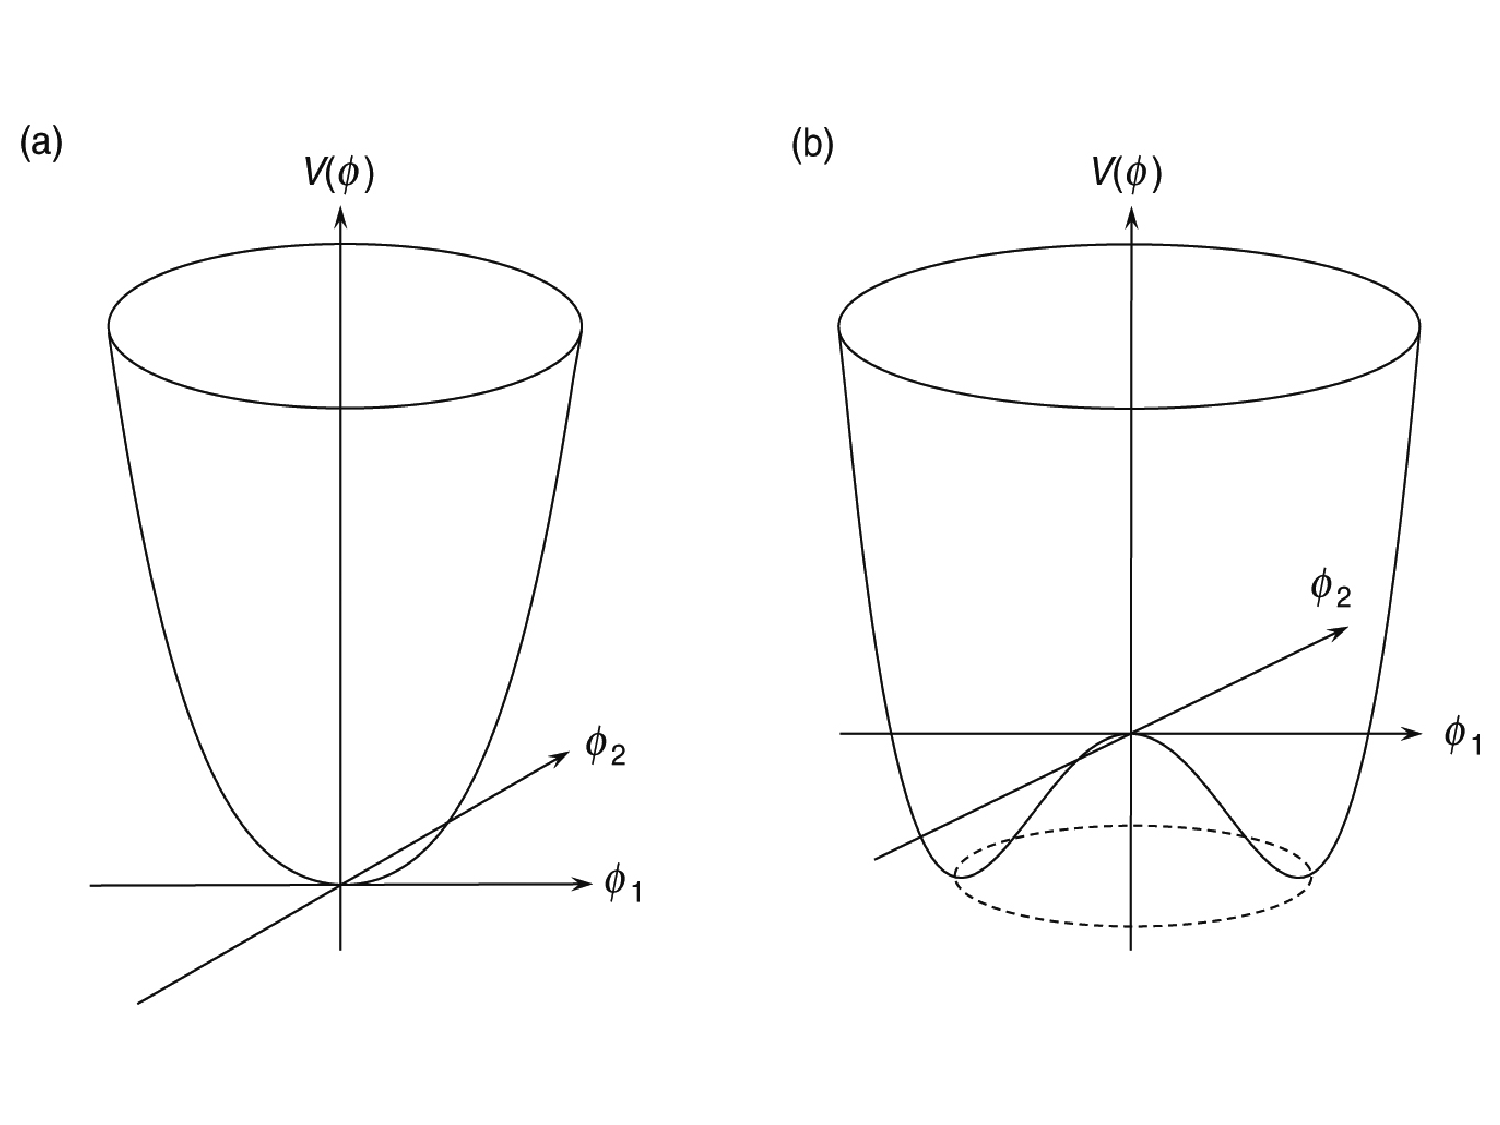
\includegraphics[width=0.8\linewidth]{figs/symm_break.pdf}
\caption{Linear sigma model potential for $N=2$. In (a) the $\phi$ field
         mass term $m^2>0$, while (b) gives this potential when
         $m^2$ is replaced by a negative parameter $-\mu^2$.
         Oscillations along the circle of minima in (b) correspond to 
         the $\pi$ field. Oscillations in the radial direction correspond
         to the $\sigma$ field. Image taken from 
         Thompson~\cite{thomson_modern_2013}.}
\label{fig:ssb}
\end{figure}

Let's try to gain some geometric intuition for this phenomenon. 
Looking at \equatref{eq:phidir}, we see that in $\phi$ space, the $\sigma$
field corresponds to oscillations of $\phi$ orthogonal to the $N-1$
dimensional hypersurface, while the massless $\pi_k$ fields
corresponds to oscillations along the hypersurface. 
An example with $N=2$ is shown in \figref{fig:ssb}. 
If we take the ground state vector~\eqref{eq:phidir} and hit it with
$\text{O}(N)$, it will be rotated somewhere else on the hypersurface.
The subgroup $\text{O}(N-1)$ hits the first $N-1$ components of the
ground state, which are all 0, thereby leaving it unchanged.
In the original $\phi^4$ theory with
$m^2>0$, the ground state vector was 0, so the $\text{O}(N)$ symmetry
was also a symmetry of the ground state. After SSB, $\text{O}(N)$ changes 
the ground state vector in general,
which is why we say the symmetry is broken. Generally any symmetry
respected by the Lagrangian but not by the ground state vector
is a broken symmetry.

In the linear sigma model, massless $\pi$ particles appeared after
SSB. This is a special example of a general result
known as Goldstone's theorem. The generated massless particles are
referred to as \index{Goldstone!boson}{\it Goldstone bosons}. 
Many light bosons can be interpreted
as approximate Goldstone bosons; as we will see in \secref{sec:cscont},
the pion can be viewed in this manner.
\begin{theorem}{Goldstone's theorem}{}
\index{Goldstone!theorem}
Consider a Lagrangian of the form
$$
  \Lagr=(\text{kinetic term for $\phi$})+
        (\text{terms independent of $\phi$})-V(\phi),
$$
where $\phi$ is the $N$-dimensional vector of real, scalar fields
$\phi_k$, and $\Lagr$ is invariant under a continuous, global
transformation of $\phi$ with generators $T^a$. Then for every
spontaneously broken generator there exists a corresponding
Goldstone boson. 
\begin{proof}
  Let $\phi_\text{min}$ be a constant field minimizing $V$. Expanding
  $V$ about this minimum we get to leading order
  $$
    V(\phi)= V(\phi_\text{min})
     +\frac{1}{2}
      (\phi-\phi_\text{min})_i(\phi-\phi_\text{min})_j\,
      \frac{\partial^2 V}{\partial\phi_i\partial\phi_j}
       \Big|_{\phi=\phi_\text{min}}.
  $$
  The differences $\phi-\phi_\text{min}$ give the new fields of the
  theory after SSB; for example in the linear sigma model this difference
  is, from \equatref{eq:phidir} and \eqref{eq:phishift},
  $$
    \phi-\phi_\text{min}=(\pi_1,...,\pi_{N-1},\sigma).
  $$
  Therefore the coefficient of the quadratic term is a symmetric matrix
  whose eigenvalues give the masses of these fields. If we can prove
  that each broken generator implies a zero eigenvalue for this matrix,
  we are done.
  The kinetic term for $\phi$ is already invariant under the global
  transformation, so if $\Lagr$ is invariant, it follows that $V$ must
  be as well. Then we can write
  $$
    V\left((\id-i\omega^aT^a)\phi\right)=V(\phi),
  $$
  where $\omega$ is some infinitesimal parameter. Expanding to linear
  order yields
  $$
    \frac{\partial V}{\partial\phi_j}(T^a\phi)_j=0.
  $$
  Differentiating the above with respect to $\phi_i$ and evaluating at
  $\phi_\text{min}$ gives
  $$
     \frac{\partial^2 V}{\partial\phi_i\partial\phi_j}
      \Big|_{\phi=\phi_\text{min}}(T^a\phi_\text{min})_j=0,
  $$
  i.e. $T^a\phi_\text{min}$ is annihilated by the mass matrix. 
  If $T^a$ is a broken generator, we have $T^a\phi_\text{min}\neq0$,
  so the above equation implies $T^a\phi_\text{min}$ is an
  eigenvector of the mass matrix with eigenvalue zero.
\end{proof}
\end{theorem}

Note that from \tabref{tab:lie}, the difference between the number of generators
of $\ON(N)$ and $\ON(N-1)$ is $N-1$, which is consistent with $N-1$ pions.


\section{Isospin and hypercharge}\label{sec:isohyper}
\index{hypercharge}\index{isospin}

We follow Chapter~9 of 
Ref.~\cite{thomson_modern_2013}. 
In quantum mechanics you learn that spin is a quantum number of
charged particles. For example the electron is a spin-1/2 particle. The
$z$-component $S_3$ of the spin operator $S$ commutes with the Hamiltonian, and
you learn that the eigenvectors of $S_3$ are the +1/2 and -1/2 states. You also
learn that the components of $S$ are related to the Pauli matrices by
\begin{equation}
  S_i=\frac{\hbar}{2}\sigma_i.
\end{equation}

Early on in nuclear physics, scientists noticed that the proton and neutron had
about the same mass, and that the nuclear force between two nucleons (i.e.
protons or neutrons) was approximately charge independent. Therefore Heisenberg
suggested that protons and neutrons were two states of a single particle (the
nucleon) just as there are spin-up and spin-down states of a spin-1/2
particle.
The quantum number corresponding to this property is called {\it isospin}.
Using this idea, the proton and neutron form an isospin doublet with total
isospin $I=1/2$ and $z$-component $I_3=\pm1/2$. Thus the Pauli matrices also
give a suitable representation of the isospin operator, and we write
\begin{equation}
  I^2=\sum\limits_{i=1}^3 I_i^2, \qquad I_i=\frac{1}{2}\sigma_i.
\end{equation}
I know this is sloppy, but I want to leave it to the reader to determine from
context whether $I$ represents the operator or the eigenvalue. 

The concept of isospin can be extended in the same way to quarks. 
In the simplest case we have $N_f=2$ and consider the lightest quarks
$u$ and $d$. The $\SU(2)$ isospin symmetry is only approximate because 
the $u$ and $d$ quarks have slightly different masses. The isospin 
doublet then has a $u$ component and a $d$ component. Generally with
$N_f$ flavors of fermion with degenerate masses, the symmetry group is 
$\SU(N_f)$ and we
form $N_f$-component multiplets in flavor space, one component per flavor.

Let's introduce the $s$ quark, assuming it has the same mass as the
$u$ and $d$ quarks, and do the $N_f=3$ case.
Using the Pauli matrices and the fact that $\SU(3)$ has 8 generators, you can
figure out what the Gell-Mann matrices are. We will say that $u$, $d$, and $s$
are eigenvectors of isospin and write
\begin{equation}
  u=\colvec{3}{1}{0}{0}, \qquad
  d=\colvec{3}{0}{1}{0}, \qquad
  s=\colvec{3}{0}{0}{1}.
\end{equation}
Then $u$ and $d$ span a 2D subspace of flavor space, so from the earlier
discussion we should know that the generators of $\SU(2)$ are contained in the
generators of $\SU(3)$. Hence
\begin{equation}
  \lambda_1=\left(\begin{array}{ccc}
            0 & 1 &  \\
            1 & 0 &  \\
              &   & 0
            \end{array}\right), \qquad
  \lambda_2=\left(\begin{array}{ccc}
            0 & -i &  \\
            i & 0  &  \\
              &    & 0
            \end{array}\right), \qquad
  \lambda_3=\left(\begin{array}{ccc}
            1 & 0  &  \\
            0 & -1 &  \\
              &    & 0
            \end{array}\right).
\end{equation}
But there's nothing special about $u$ and $d$; $u$ and $s$ will similarly form
a subspace, and so will $d$ and $s$. In both cases, we will use the Pauli
matrices as generators. We can similarly write
\begin{equation}
  \lambda_4=\left(\begin{array}{ccc}
            0 &   & 1\\
              & 0 &  \\
            1 &   & 0
            \end{array}\right), \qquad
  \lambda_5=\left(\begin{array}{ccc}
            0 &    & -i \\
              & 0  &    \\
            i &    & 0
            \end{array}\right), \qquad
  \lambda_X=\left(\begin{array}{ccc}
            1 &    & 0 \\
              & 0  &   \\
            0 &    & -1
            \end{array}\right),
\end{equation}
\begin{equation}
  \lambda_6=\left(\begin{array}{ccc}
            0 &   &  \\
              & 0 & 1\\
              & 1 & 0
            \end{array}\right), \qquad
  \lambda_7=\left(\begin{array}{ccc}
            0 &    &   \\
              & 0  & -i\\
              & i  & 0
            \end{array}\right), \qquad
  \lambda_Y=\left(\begin{array}{ccc}
           0  &    &  \\
              & 1  & 0\\
              & 0  & -1 
            \end{array}\right).
\end{equation}
Finally note the fact that there are only 8 linearly independent generators, so
two of these matrices should be linearly dependent. Since the
$u\leftrightarrow d$ isospin symmetry is the closest to being exact, we choose
the last generator to be a linear combination of $\lambda_X$ and $\lambda_Y$
that treats the $u$ and $d$ quarks symmetrically. Thus
\begin{equation}
  \lambda_8=\frac{1}{\sqrt{3}}\lambda_X+\frac{1}{\sqrt{3}}\lambda_Y
           =\frac{1}{\sqrt{3}}\left(\begin{array}{ccc}
            1 &   &   \\
              & 1 &   \\
              &   & -2
            \end{array}\right).
\end{equation}
The new isospin and total isospin operators are
\begin{equation}
  I^2=\frac{1}{4}\sum\limits_{i=1}^8 I_i^2, \qquad I_i=\frac{1}{2}\lambda_i.
\end{equation}

In the case of $\SU(2)$, the operators $I_i$ do not commute, and therefore are
not simultaneously diagonalizable. For $\SU(3)$ in the Gell-Mann basis,
$I_3$ and $I_8$ are both diagonal, so they correspond to compatible
observables. The observable $I_3$ is itself sometimes referred to
as isospin or weak isospin. The observable we associate with $I_8$ is rescaled as
\begin{equation}
  Y=\frac{1}{\sqrt{3}}\lambda_8,
\end{equation}
and $Y$ is called the {\it hypercharge}.\index{hypercharge} 
We can quickly obtain the isopins and hypercharges of
our lightest quarks: 
\begin{equation}\begin{aligned}
\hat{I_3}\,u =\frac{1}{2}u ~~~ &\text{and}~~~\hat{Y}u=\frac{1}{3}u,\\
\hat{I_3}\,d =-\frac{1}{2}d ~~~ &\text{and}~~~\hat{Y}d=\frac{1}{3}d,\\
\hat{I_3}\,s = 0           ~~~ &\text{and}~~~\hat{Y}s=-\frac{2}{3}s.
\end{aligned}\end{equation}
One can summarize this pattern of conserved charges in the following formula:
\begin{theorem}{Gell-Mann-Nishijima Formula}{}
\index{Gell-Mann-Nishijima formula}
  The electric charge $Q$ of a particle is related to its isospin and
  hypercharge by
  \begin{equation*}
    Q=I_3+\frac{1}{2}Y
  \end{equation*}
\end{theorem}


\section{Chiral symmetry}\label{sec:cscont}
\index{chiral symmetry}

There are some interesting, approximate global symmetries of the QCD Lagrangian
that crop up in the limit of zero quark mass. They are related to isospin
discussed in \secref{sec:isohyper}. Introducing small quark masses breaks this
symmetry; hence from the perspective of an effective theory of bound states we
can find something like Goldstone bosons in accordance with the discussion in
\secref{sec:ssb}. 
In this section we work with a Euclidean metric. We follow
Chapter 7 of Gattringer and
Lang~\cite{gattringer_quantum_2010}.

The massless fermion action for a single flavor reads
\begin{equation}
S_F=\int\dd[4]{x}\Lagr_F=\int\dd[4]{x}\bar{\psi}\slashed{D}\psi. 
\end{equation}
We refer to $\slashed{D}$ as the {\it massless Dirac operator}. A
\index{rotation!chiral}
{\it chiral rotation}\footnote{You may notice that the sign in the exponent
is the same for both the spinor field and its conjugate field. This is a
common feature whenever a $\gamma_5$ is in the exponent. Recall that
$\bar{\psi}=\psi^\dagger\gamma_4$. The $\gamma_5$ will anticommute with
$\gamma_4$.} of the fermion fields is a transformation
mapping
\begin{equation}
  \psi\to e^{i\alpha\gamma_5}\psi~~~~\text{and}~~~~
  \bar{\psi}\to\bar\psi e^{i\alpha\gamma_5},
\end{equation}
where $\alpha\in\R$. This is called a chiral rotation
because $\gamma_5$, which is used to define the operators~\eqref{eq:projdef},
projects out the left-handed and right-handed components of the
fermion field according to \equatref{eq:projact}. 
Using identity 2 of
\propref{prp:gammatech}, we find that $\Lagr_F$ transforms under this
rotation as
\begin{equation}
  \Lagr_F\to\bar{\psi}e^{i\alpha\gamma_5}\slashed{D}e^{i\alpha\gamma_5}\psi
         =\bar{\psi}e^{i\alpha\gamma_5}e^{-i\alpha\gamma_5}\slashed{D}\psi
         =\Lagr_F,
\end{equation}
i.e. it is invariant under chiral rotations. Using
\propref{prp:projection}, one can decompose $\Lagr_F$ into its
left-handed and right-handed parts as
\begin{equation}
  \Lagr_F=\bar{\psi}_L\slashed{D}\psi_L
         +\bar{\psi}_R\slashed{D}\psi_R,
\end{equation}
and we colloquially say that the chiral components of
$\Lagr_F$ ``do not talk to each other."
If one were to include a mass term in $\Lagr_F$, it would decompose as
\begin{equation}
  m\bar{\psi}\psi=m\left(\bar{\psi}_R\psi_L+\bar{\psi}_L\psi_R\right),
\end{equation}
which mixes the chiral components, thereby breaking chiral symmetry.
\index{limit!chiral}
This is why one refers to the limit $m\to0$ as the {\it chiral limit}.


We now generalize these ideas to $N_f$ flavors of fermion.
In general we can write a fermion action as
\begin{equation}\label{eq:nfact}
  S_F=\int\dd[4]{x}\Lagr_F=\int\dd[4]{x}
         \bar{\psi}\left(\slashed{D}+M\right)\psi,
\end{equation}
where $M$ is the {\it mass matrix}\index{mass matrix}
\begin{equation}
  M~``="~\diag(m_1,m_2,...,m_{N_f})
\end{equation}
acting in flavor space. Here the $\psi$ can be thought of as a vector with $N_f$
components $\psi_f$ like
\begin{equation}
  \psi=\colvec{4}{\psi_1}{\psi_2}{\vdots}{\psi_{N_f}}.
\end{equation}
Each $\psi_f$ is a 4-component Dirac spinor, and so $M$ has the form 
\begin{equation}
  M=\left(\begin{array}{cccc}
      m_1\id_4 &          &        & \\
               & m_2\id_4 &        & \\
               &          & \ddots & \\
               &          &        & m_{N_f}\id_4
    \end{array}\right).
\end{equation}
Similarly when we write $\gamma_\mu$ in \equatref{eq:nfact} what we really mean is
\begin{equation}
  \gamma_\mu
            =\left(\begin{array}{cccc}
               \gamma_\mu &            &        & \\
                          & \gamma_\mu &        & \\
                          &            & \ddots & \\
                          &            &        & \gamma_\mu
               \end{array}\right).
\end{equation}
Where the $\gamma^\mu$ in the matrix are defined as usual while the $\gamma_\mu$
on the LHS is just a shorthand. I'm sorry about this confusing notation. 

In the chiral limit, the action \equatref{eq:nfact} is again invariant under
\index{rotation!axial vector}
{\it axial} rotations taking the form
\begin{gather}
  \label{eq:SUNfc}
  \psi\to e^{i\gamma_5\alpha^a T^a}\psi,\qquad
    \bar{\psi}\to\bar{\psi}e^{i\gamma_5\alpha^a T^a}, \\
  \label{eq:U1A}
  \psi\to e^{i\alpha\gamma_5 \id}\psi,\qquad
    \bar{\psi}\to\bar{\psi}e^{i\alpha\gamma_5 \id},
\end{gather}
where the $T^a$ are the $N_f^2-1$ generators of $\SU(N_f)$,
$\id\equiv\id_{4N_f}$, and again $\alpha^a,\alpha\in\R$.
In this limit the action is also invariant under 
the \index{rotation!vector}{\it vector rotations}
\begin{gather}
  \label{eq:SUNf}
  \psi\to e^{i\alpha^a T^a}\psi,\qquad
    \bar{\psi}\to\bar{\psi}e^{-i\alpha^a T^a}, \\
  \label{eq:U1V}
  \psi\to e^{i\alpha \id}\psi,\qquad
    \bar{\psi}\to\bar{\psi}e^{-i\alpha \id}.
\end{gather}
The corresponding Noether currents for these symmetries are, up to a sign,
respectively
\begin{equation}\begin{aligned}
J^{5a}_\mu&=\psibar T^a\gamma_\mu\gamma^5\psi,\\
J^5_\mu&=\psibar\gamma_\mu\gamma^5\psi,\\
J^a_\mu&=\psibar T^a\gamma_\mu\psi,\\
J_\mu&=\psibar\gamma_\mu\psi.\\
\end{aligned}\end{equation}

Using eqs.~\eqref{eq:SUNfc} and \eqref{eq:SUNf}, we can define a general
chiral rotation\index{rotation!chiral} by
\begin{equation}\label{eq:chiralRotation}
  \psi\to e^{i(\alpha^a + \gamma_5\beta^a)T^a}\psi.
\end{equation}
If we take $\beta^a=0$ in \equatref{eq:chiralRotation}, we get the diagonal
isospin subgroup.
If we express the action~\eqref{eq:nfact} in terms of left-handed and
right-handed components of $\psi$, we will find that, in the chiral limit, the 
rotation~\eqref{eq:chiralRotation} can be decomposed into two $\SU(2)$
rotations, one rotating the left-handed fields of different flavors
among themselves and similarly for right-handed fields. This reflects
\begin{equation}
\SU(2)_V\times\SU(2)_A = \SU(2)_L\times\SU(2)_R.
\end{equation}

The invariance under eqs.~\eqref{eq:SUNf} and \eqref{eq:U1V} extends to the case of degenerate
masses, when $m_1=m_2=...=m_{N_f}\equiv m$, and is the familiar isospin
symmetry generalized to $N_f$ flavors. The symmetry~\eqref{eq:U1V} holds for
\index{baryon number}
arbitrary masses, and the corresponding Noether current suggests
the conserved quantity in QCD is the 
{\it baryon number}\footnote{You can see why it's called baryon number: 
A baryon is made of 3
quarks, and hence has $B=1$. Anti-quarks have $B=-1$, and
mesons have $B=0$.}
\begin{equation}
    B=\frac{1}{3}(n_q-n_{\bar{q}}).
\end{equation}


Returning once again to the massless limit, the invariance of the action under
\equatref{eq:SUNfc}, \eqref{eq:U1A}, \eqref{eq:SUNf}, and \eqref{eq:U1V}
represents the global symmetry group
\begin{equation}\label{eq:SMfglobal}
  \SU(N_f)_L\times\SU(N_f)_R\times\U(1)_V\times\U(1)_A.
\end{equation}
Breaking the global symmetry group~\eqref{eq:SMfglobal} has important
implications in QCD phenomenology. For example we will show that in the
quantized, massless theory the fermion determinant changes
under~\equatref{eq:U1A}, breaking the $\U(1)_A$ symmetry explicitly. The remaining
symmetry is
\begin{equation}\label{eq:SMglobalbUA}
  \SU(N_f)_L\times\SU(N_f)_R\times\U(1)_V.
\end{equation}
If the fermion masses are degenerate, the symmetry $\SU(N_f)_L\times\SU(N_f)_R$
breaks to its subgroup $\SU(N_f)_V$. Now the remaining symmetry is
\begin{equation}
  \SU(N_f)_V\times\U(1)_V.
\end{equation}
Finally allowing non-degenerate masses breaks the symmetry further.
There remains
\begin{equation}
  \underbrace{\U(1)_V\times\U(1)_V\times...\times\U(1)_V}_\text{$N_f$ times}.
\end{equation}

The typical QCD scale\footnote{Think of protons, which have a mass of about
940~MeV.} is $\sim1~\text{GeV}$ 
so the $u$, $d$, and $s$ quarks have masses that
are relatively small (about 5~MeV, 5~MeV, and 100~MeV, respectively).
Since these masses are so close to zero on this scale, we can say that
when $N_f=2$, and partly for $N_f=3$, \equatref{eq:SMglobalbUA} is
an approximate symmetry. If the $u$ and $d$ quarks were massless, this symmetry
would be exact, and it can be argued~\cite{gattringer_quantum_2010} that
a nucleon and its negative parity partner should have the same mass.
However one finds the negative parity nucleon to have
a mass of about 1535~MeV, and this difference of about 600~MeV is too large to
be explained by the slight breaking due to the $u$ and $d$ masses. We
conclude that something else is happening. This is another example
of SSB: If quarks were massless, the pions would arise as
the Goldstone bosons of chiral SSB; hence we refer to pions as
``would-be" Goldstone bosons.

\subsection{Chiral perturbation theory}

Let us try to understand the situation with only two light quarks $u$ and $d$.
As discussed above, introducing massive, degenerate fermions introduces a
symmetry-breaking pattern
\begin{equation}
\SU(2)_L\times\SU(2)_R\to\SU(2)_V,
\end{equation}
which is the isospin symmetry. Inspired by Goldstone's theorem, we would like to
find an effective model in which this symmetry-breaking pattern lets us clearly see
the pions as Goldstone bosons. We will use the linear sigma model as guide.
This presentation follows Ref.~\cite{schwartz_quantum_2014}.

Let $g_L\in\SU(2)_L$ and $g_R\in\SU(2)_R$. We introduce scalar fields
$\sigma_{ij}(x)$ that transform under $\SU(2)_L\times\SU(2)_R$ as
\begin{equation}\label{eq:chiralPertRot}
\Sigma\to g_L\Sigma g_R^\dagger,\qquad
\Sigma^\dagger\to g_R\Sigma^\dagger g_L^\dagger.
\end{equation}
An effective Lagrangian for this field is given by the linear sigma model
\begin{equation}
\Lagr=\left|\partial_\mu \Sigma\right|^2+m^2|\Sigma|^2-\frac{\lambda}{4}|\Sigma|^4,
\end{equation}
where $|\Sigma|^2=\Sigma_{ij}\Sigma^\dagger_{ji}$. This Lagrangian is invariant
under the rotations~\eqref{eq:chiralPertRot}. The potential part is minimized
when
\begin{equation}
\ev{\Sigma_{ij}}=\frac{v}{\sqrt{2}}\id_2,
\end{equation}
where the scale for the VEV is $v=\sqrt{m/2\lambda}$ like before.
This choice corresponds to $\SU(2)_L\times\SU(2)_R$ breaking down
to $\SU(2)_V$. 

Next we define shifted fields $\pi^a$ and $\sigma$ relative to this point.
This time we write it as
\begin{equation}
\Sigma(x)=\frac{v+\sigma(x)}{\sqrt{2}} \exp \left(2 i \frac{\pi^a(x) \tau^a}{f_\pi}\right)
\end{equation}
with the {\it pion decay constant}\index{decay constant!pion} $f_\pi$ given by
\begin{equation}
f_\pi=\frac{2m}{\lambda}=v,
\end{equation}
which leads to a nice normalization for the pion kinetic terms.
In the limit $m\to\infty$ and $\lambda\to\infty$ holding $f_\pi$ fixed we get
\begin{equation}\label{eq:Udef}
\frac{\sqrt{2}}{v} \Sigma(x) \rightarrow U(x) \equiv \exp 
\left[2 i \frac{\pi^a \tau^a}{f_\pi}\right]=\exp \left[\frac{i}{f_\pi}
\left(\begin{array}{cc}
\pi^0 & \sqrt{2} \pi^{-} \\
\sqrt{2} \pi^{+} & -\pi^0
\end{array}\right)
\right],
\end{equation}
where $\pi^0=\pi^3$ and $\pi^\pm=(\pi^1\pm i\pi^2)\sqrt{2}$. This matrix form is
thus determined by $\SU(2)$. Note that $U^\dagger U=\id$. Furthermore it
transforms under $\SU(2)_L\times\SU(2)_R$ as
\begin{equation}
U\to g_LU g_R^\dagger.
\end{equation}

Let us now write down the most general Lagrangian involving $U$ invariant under 
$\SU(2)_L\times\SU(2)_R$. It is 
\begin{equation}\begin{aligned}\label{eq:chiralLagr}
\Lagr_\chi=\frac{F_\pi^2}{4} \operatorname{tr}\left[\left(D_\mu U\right)\left(D_\mu U\right)^{\dagger}\right] & +L_1 \operatorname{tr}\left[\left(D_\mu U\right)\left(D_\mu U\right)^{\dagger}\right]^2 \\
&+L_2 \tr \left[\left(D_\mu U\right)\left(D_\nu U\right)^{\dagger}\right] \operatorname{tr}\left[\left(D_\nu U\right)^{\dagger}\left(D_\mu U\right)\right]  \\
& +L_3 \tr\left[\left(D_\mu U\right)\left(D_\mu
U\right)^{\dagger}\left(D_\nu U\right)\left(D_\nu U\right)^{\dagger}\right]\\
&+\cdots
\end{aligned}\end{equation}
This is the {\it chiral Lagrangian}\index{chiral Lagrangian}. This form is
determined by the fact we need pairs of $g_L$ and $g_R$ to cancel. Every term
requires derivatives since terms like $U^\dagger U$ are constant and hence have
no influence on the equations of motion.
In general these covariant derivatives include EW gauge fields, but no gluons.

Plugging \equatref{eq:Udef} into \equatref{eq:chiralLagr} and expanding the
exponential we find
\begin{equation}\begin{aligned}
& \frac{F_\pi^2}{4} \tr\left[\left(D_\mu U\right)\left(D_\mu U\right)^{\dagger}\right]
=\frac{1}{2}\left(\partial_\mu \pi^0\right)\left(\partial_\mu \pi^0\right)+\left(D_\mu \pi^{+}\right)\left(D_\mu \pi^{-}\right)^{\dagger} \\
& \quad+\frac{1}{F_\pi^2}\left[-\frac{1}{3} \pi^0 \pi^0 D_\mu \pi^{+} D_\mu
\pi^{-}+\cdots\right]+\cdots
\end{aligned}\end{equation}
We thus find an expansion in powers of $f_\pi^{-2}$. This implies terms $L_i$ in
\equatref{eq:chiralLagr} are suppressed relative to the leading term.
Note that there is no pion mass term, which is consistent with them being
Goldstone bosons.

\subsection{The GMOR formula}

In this section we derive a relation between pion masses and $u$ and $d$ masses.
Chiral perturbation theory gives us a lot of useful information about pion
interactions and their interactions with the EW sector, which motivates it as a
possible starting point. The trouble is we have no pion mass term, and the
theory does not know about $u$ and $d$ quarks.

To extend $\Lagr_\chi$ to include $u$ and $d$ masses, we consider a term
\begin{equation}
\Lagr_{ud}=\psibar M \psi, \quad M=\left(\begin{array}{cc}
m_u & 0 \\
0 & m_d
\end{array}\right)
\end{equation}
with $\psi$ containing $u$ and $d$ quarks only. To avoid trashing our
$\SU(2)_L\times\SU(2)_R$ symmetry, we treat the constants $m_u$ and $m_d$ as
fields and demand that the matrix $M$ transform as
\begin{equation}
M\to g_LMg_R^\dagger.
\end{equation}
Constants treated as fields in this way are sometimes called {\it
spurions}\index{spurion}. 

\begin{figure}
\centering
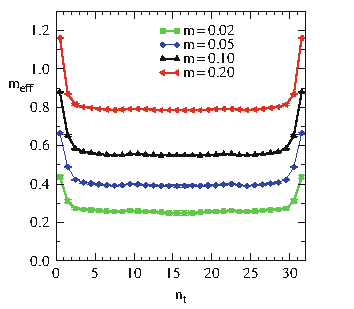
\includegraphics[width=0.5\linewidth]{figs/GMOR.pdf}
\caption{Effective pion mass extracted from pion correlation functions
for a $32^3\times16$ lattice calculation at $a\approx0.15$ fm.
Results given for different bare light quark masses. Connecting lines guide the
eye. Image taken from Ref.~\cite{gattringer_quantum_2010}.}
\label{fig:GMOR}
\end{figure}

Now we cannot include the term $\Lagr_{ud}$ directly because this is a theory
where pions are the effective degrees of freedom, not the quarks. However we can
include terms with $M$ to see what happens. The leading term we can add to
$\Lagr_\chi$ looks like
\begin{equation}
\begin{aligned}
\Lagr_M & =\frac{V^3}{2} \operatorname{tr}\left(M U+M^{\dagger} U^{\dagger}\right) \\
& =V^3\left(m_u+m_d\right)-\frac{V^3}{2
F_\pi^2}\left(m_u+m_d\right)\left(\pi_0^2+\pi_1^2+\pi_2^2\right)+\order{\pi^3} .
\end{aligned}
\end{equation}
The prefactor $V^3/2$ was picked so that the VEV from $\Lagr_M$ matches the VEV
from $\Lagr_{ud}$; here $V^3=\ev{\bar{u}u}=\ev{\bar{d}d}$. Looking at coupling
for the $\pi^2$ terms, we read off the pion mass as
\begin{equation}
  M_\pi^2\approx \frac{V^3}{f_\pi^2}(m_u+m_d).
\end{equation}
This is the Gell-Mann-Oakes-Renner (GMOR)
formula~\cite{gell-mann_behavior_1968}.
It directly shows that the pion mass is not simply the sum of
the valence quark masses. Moreover since you know the physical values
of $M_\pi$, $m_u$, and $m_d$, this equation can be used to crudely estimate
$M_\pi$ for unphysical light quark masses.

In \figref{fig:GMOR} we show the results of a lattice calculation of the pion
mass taken from Ref.~\cite{gattringer_quantum_2010}. Note that increasing the
bare mass from 0.02 to 0.05 leads to a change in $m_\text{eff}$ of
$0.4/0.26\approx1.54$. From the GMOR formula, we would expect the pion mass to
change by a factor $\sqrt{0.05/0.02}\approx1.58$. Hence we see that the GMOR
formula holds to good accuracy also in lattice QCD.

\section{Anomalous magnetic moment}\label{sec:magAnom}
The {\it magnetic moment}\footnote{This is the dipole contribution to the
magnetic moment. Higher order moments, such as the quadrupole, are forbidden.
In particular this multipole expansion, which can be expressed in
terms of spherical harmonics $Y_l^m$, has its $l$ limited to $l=1$
since the only particles we consider are spin-1/2.}\index{magnetic moment} 
of a particle $X$, $\vec{M}_X$,
with $X\in\{e,\mu,\tau\}$
determines how it responds to an external magnetic field $\vec{B}$. In particular it
gives a contribution to the energy $-\vec{M}_X\cdot\vec{B}$.
The magnetic moment itself comes from the particle's intrinsic spin $\vec{S}_X$,
\begin{equation}
  \vec{M}_X=g_X\frac{q_X}{2m_X}\vec{S}_X,
\end{equation}
where $g_X$ is a constant called the {\it g-factor}\index{g-factor}
or {\it gyromagnetic ratio}\index{gyromagnetic ratio} and
$m_X$ and $q_X$ are the particle's mass and charge, respectively.
Using relativistic quantum mechanics, one can argue $g_X=2$. Any
deviation from 2 is thus called the {\it anomalous magnetic moment},
\index{magnetic moment!anomalous}
\begin{equation}
  a_X=\frac{g_X-2}{2}.
\end{equation}


\subsection{Vacuum polarization}\label{sec:VP}\index{vacuum polarization}

For this section we closely follow Ref.~\cite{maiani_hadron_2016}, 
which I found to be quite
a nice introduction to vacuum polarization.

The simplest case of {\it vacuum polarization} (VP) is a one-loop effect in
$e^+e^-$ scattering in QED. If the virtual photon has enough energy,
an $e^+e^-$ pair can be emitted and reabsorbed, and this
pair will effectively screen\footnote{The name can be remembered in analogy to
the application of an external magnetic field on a dielectric material.
In this case the polarized molecules in the material will also screen
the external field inside the material.} the electromagnetic field, reducing the force
carried by the photon.

\begin{figure}
\centering
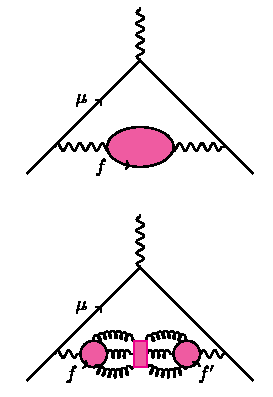
\includegraphics[width=0.8\linewidth]{figs/HVP.pdf}
\caption{HVP contribution to $a_\mu$. It arises from the two
contributions shown in this figure. {\it Top}: Quark-line
connected contribution, which is a virtual quark
bubble inserted in photon propagator. {\it Bottom}:
Quark-line disconnected contribution, which consists of
virtual quark bubbles connected by gluons. The bubbles
include all possible QED interactions.
Image taken from Ref.~\cite{FermilabLattice:2022izv}.}
\label{fig:HVPmuon}
\end{figure}


Any possible charged particle-antiparticle pair must be considered,
for instance $\mu^+\mu^-$ and $\tau^+\tau^-$. Their effects are small compared
to $e^+e^-$ due to their comparatively large masses, and are hence
only noticeable for large\index{virtuality} {\it virtuality}, or $q^2$,
of the exchanged photon. 
Contributions to VP coming from strongly interacting particles
is referred to as\index{vacuum polarization!hadronic} 
{\it hadronic vacuum polarization} (HVP).
Their effect can be computed perturbatively at large $q^2$,
but at small $q^2$ this of course fails.
The HVP contribution to $a_\mu$ is shown in \figref{fig:HVPmuon}.

The first experimental indication of HVP was found at 
LAL-Orsay~\cite{augustin_evidence_1973},
which measured the cross section for $e^+e^-\to\mu^+\mu^-$.
There a characteristic interference pattern was found for
the $\phi(1020)$ resonance\footnote{A {\it phi meson} $\phi$
is\index{meson!f@$\phi$} a strange-antistrange pair.}, in concordance with the
$\phi$ HVP contribution. CERN had a series of experiments
starting in 
1958~\cite{charpak_measurement_1961,bailey_precise_1971,bailey_anomalous_1977}, 
culminating in a measurement of $a_\mu$, which agreed at the time with the 
SM~\cite{calmet_anomalous_1977}.


Since then, higher precision was achieved at Brookhaven
and J-PARC, and a state-of-the-art determination from 
Fermilab~\cite{abi_measurement_2021}
places experimental searches at 4.2$\sigma$ tension
against data-driven theoretical methods,
which we will discuss shortly~\cite{aoyama_anomalous_2020}.


At the same time that this 4.2$\sigma$ tension was revealed,
the BMW collaboration offered a lattice calculation with precision competitive
with data-driven approaches~\cite{borsanyi_leading_2021}.
Their result tantalizingly lies between the data-driven result and experiment,
being about 2.1$\sigma$ above the theory and 1.6$\sigma$ below experiment.
Understanding this 3-fold tension requires careful investigation of
systematics. We will discuss the lattice perspective
in more detail in \secref{sec:muonAnom}. 



\section{Thirring model}\label{sec:Thirring}\index{Thirring model}

The {\it Thirring model}~\cite{thirring_soluble_1958} is a QFT in 1+1 dimensions.
Its Lagrangian density is given by
\begin{equation}
  \Lagr=\bar{\psi}(i\partial\!\!\!/-m)\psi -\frac{g}{2}
         \left(\bar{\psi}\gamma_\mu\psi\right) \left(\bar{\psi}\gamma^\mu
\psi\right),
\end{equation}
where here $\gamma^\mu$ are 2-$d$ gamma matrices.
This describes a Dirac field with a self-interaction.
What's special about the massless Thirring model is that it is 
exactly solvable~\cite{johnson_solution_1961,hagen_new_1967,klaiber_1968}, 
which means it is a useful test bed for various QFT methods.
The massive Thirring model is partially solvable: my understanding is that the
correlations are not yet known.

In the context of lattice calculations, the Thirring model is used often as a
test bed for Lefshetz thimbles, which are a possible sign problem workaround.
Sometimes in these studies, one may consider a model with more or fewer spatial
dimensions.

\section{Gross-Neveu model}\label{sec:GNmodel}\index{Gross-Neveu model}

The {\it Gross-Neveu model} \cite{gross_dynamical_1974} is another
1+1 dimensional, toy QFT model. It contains $N$ Dirac fermions with a
4-fermion vertex. Some nice features of this model include that it is
asymptotically free and has a dynamical mass generation mechanism, making
a good QCD toy model. This Lagrangian density is given by
\begin{equation}
\Lagr=\bar{\psi}^a(i \slashed\partial-m) \psi^a+\frac{g^2}{2
N}\left(\bar{\psi}^a \psi^a\right)^2,
\end{equation}
where $1\leq a\leq N$.

\section{Topological invariants}\label{sec:topinvar}\index{topological!winding number}

This section follows Chapter 93 of Srednicki~\cite{srednicki_quantum_2007};
more details can be found there.
We start by considering classical, Euclidean, pure $\SU(2)$ gauge theory
\begin{equation}\label{eq:topaction}
  \Lagr=-\frac{1}{2g^2}F_{\mu\nu}F_{\mu\nu}
\end{equation}
at fixed $x_4$, focusing for the moment on $U$ that are time-independent.
Let $U\equiv U(\vec{x})\in\SU(2)$, and set the BC $U(\infty)=U_0$
for some constant matrix $U_0$.
The {\it topological winding number}
or {\it Pontryagin index} \index{Pontryagin index}of the map $U$ is
\begin{equation}\label{eq:wn}
  n\equiv\frac{1}{24\pi^2}\int\dd[3]{x}\epsilon_{ijk}
    \tr U\,\partial_iU^\dagger U\,\partial_jU^\dagger
        U\,\partial_kU^\dagger.
\end{equation}
The winding number is invariant under coordinate changes since the Jacobian of
the measure cancels the Jacobian of the partial derivatives.
Given the BC, it is also invariant under smooth deformations of $U$.
To show this, we first establish a useful Lemma.

\begin{lemma}{}{variationrule}
  $$\var\left(U\partial_kU^\dagger\right)
   =-U\partial_k\left(U^\dagger\var U\right)U^\dagger.$$
\begin{proof} Note that $\var U^\dagger=-U^\dagger\var U\,U^\dagger$. Hence
  \begin{alignat*}{2}
   \var\left(U\partial_kU^\dagger\right)
    &=\var U\partial_kU^\dagger&&+U\partial_k\var U^\dagger\\
    &=                           &&-U\partial_k\left(U^\dagger\var
                                                     U\,U^\dagger\right)\\
    &=                           &&-U\left(\partial_kU^\dagger\var UU^\dagger
                                        +U^\dagger\partial_k\var U\,U^\dagger
                                        +U^\dagger\var U\partial_k
                                         U^\dagger                     \right).
  \end{alignat*}
  Cancelling the first and last terms and using the product rule gives the
  result.
\end{proof}
\end{lemma}

\begin{theorem}{}{wndeform}
The topological winding number is invariant under smooth
deformations of $U$.
\begin{proof} We integrate \equatref{eq:wn} over a time-slice of space-time,
which we call $\Omega$. Then
  \begin{align*}
   \var n &=-\frac{1}{24\pi^2}~\var\int_\Omega\dd[3]{x}\epsilon_{ijk}\tr
                U\partial_iU^\dagger\,
                U\partial_jU^\dagger\,
                U\partial_kU^\dagger\\
            &=-\frac{1}{8\pi^2}\int_\Omega \dd[3]{x}\epsilon_{ijk}\tr
                \var\left(U\partial_iU^\dagger\right)
                            U\partial_jU^\dagger\,
                            U\partial_kU^\dagger\\
            &=+\frac{1}{8\pi^2}\int_\Omega \dd[3]{x}\epsilon_{ijk}\tr
                \partial_i\left(U^\dagger\var U\right)
                 U^\dagger\partial_jU\,
                 U^\dagger\partial_kU\\
           &=+\frac{1}{8\pi^2}\int_{\partial\Omega} \dd{S_i}\epsilon_{ijk}\tr
                U^\dagger\var U\,
                U^\dagger\partial_j U\,
                U^\dagger\partial_k U\\
            &~~~~~-\frac{1}{8\pi^2}\int_\Omega \dd[3]{x}\epsilon_{ijk}\tr
                U^\dagger\var U\partial_i\left[
                U^\dagger\partial_j U\,
                U^\dagger\partial_k U\right].
  \end{align*}
  In the second step we used the product rule and the fact that the trace 
  and Levi-Civita symbols are cyclic.
  In the third step we used \lemref{lem:variationrule} as well as
  $U\partial_\mu U^\dagger=-\partial_\mu UU^\dagger$. In the last step
  we integrated by parts. The first integral is over the time-slice boundary
  evaluated at infinity. Since $\partial_jU=\partial_jU_0=0$ there, this term
  vanishes. The integrand of the remaining integral is expanded as
  \begin{equation*}\begin{aligned}
    \epsilon_{ijk}\tr\Big[&
     \partial_i U^\dagger\partial_j U U^\dagger\partial_k U
     +\partial_j U^\dagger\partial_i U U^\dagger\partial_k U\\
     &+U^\dagger\partial_{ij}UU^\dagger\partial_k U
     +U^\dagger\partial_jUU^\dagger\partial_{ik}U\Big].
  \end{aligned}\end{equation*}
  Terms with double derivatives vanish, as they are symmetric with respect
  to exchange of indices, while $\epsilon$ is antisymmetric. The remaining
  terms are also shown to vanish using the antisymmetry of $\epsilon$
  in addition to cyclically permuting terms under the trace.
\end{proof}
\end{theorem}

The quantity~\eqref{eq:wn} is called a winding number because it counts
the number of times the mapping $U$ ``winds around" or ``covers" 
the integration region. Let us see how this works in the present case.
The integration region is the 3D surface of space-time, which is
homeomorphic to the 3-sphere $S^3$. A point $\hat{x}\in S^3$
is specified by two polar angles $\chi$ and $\psi$ and an azimuthal
angle $\phi$ as
\begin{equation}
  \hat{x}=\colvec{4}{\s_\chi\s_\psi\co_\phi}{\s_\chi\s_\psi\s_\phi}
                    {\s_\chi\co_\psi}{\co_\chi}.
\end{equation}
Then the mapping $U:S^3\to\SU(2)$ given by
\begin{equation}\label{eq:uexplicit}
U(\hat{x})=\left(\begin{array}{cc}
             \co_\chi+i\s_\chi\co_\psi     & i\s_\chi\s_\psi e^{-im\phi}\\
             i\s_\chi\s_\psi e^{im\phi}& c_\chi-i\s_\chi\co_\psi 
            \end{array}\right),
\end{equation}
has winding number $m$. Intuitively, one can see this in the following manner:
Any $\SU(2)$ matrix can be written in terms of four real components as 
\begin{equation}
  U=a_4\id+i\vec{a}\cdot\vec{\sigma},
\end{equation}
where $a_\mu a_\mu=1$. The vector corresponding to the 
map~\eqref{eq:uexplicit} is
\begin{equation}
  \hat{a}=\colvec{4}{\s_\chi\s_\psi\co_{m\phi}}{\s_\chi\s_\psi\s_{m\phi}}
                    {\s_\chi\co_\psi}{\co_\chi}.
\end{equation}
We see that if we sweep through $\phi$, $\hat{x}$ sweeps over $S^3$ once
while $\hat{a}$ sweeps over $S^3$ $m$ times. And indeed, one can see
that \equatref{eq:wn} extracts the winding number by plugging in the 
mapping~\eqref{eq:uexplicit}. This is done in the following Proposition.

\begin{proposition}{}{wnproof}
Consider the map $U:S^3\to\SU(2)$ given by
$$
U(\hat{x})=\left(\begin{array}{cc}
             \co_\chi+i\s_\chi\co_\psi     & i\s_\chi\s_\psi e^{-im\phi}\\
             i\s_\chi\s_\psi e^{im\phi}& c_\chi-i\s_\chi\co_\psi 
            \end{array}\right).
$$
Then $U$ has winding number $m$.
\begin{proof}
  Plugging this map into \equatref{eq:wn} we find
  \begin{equation*}
  \begin{aligned}
    n&=-\frac{1}{24\pi^2}\int_{S^3} \dd[3]{x}\epsilon_{ijk}\tr
        U\partial_i U^\dagger\,U\partial_j U^\dagger\,U\partial_k U^\dagger\\
   &=-\frac{1}{24\pi^2}\int_0^\pi\dd\chi\int_0^\pi\dd{\psi}\int_0^{2\pi}
        \dd{\phi}\epsilon_{\alpha\beta\gamma}\tr
        U\partial_\alpha U^\dagger\,U\partial_\beta U^\dagger\,
        U\partial_\gamma U^\dagger,\\
  \end{aligned}
  \end{equation*}
  where $\alpha,\,\beta,\,\gamma\in\{\chi,\,\psi,\,\phi\}$ and
  $\epsilon_{\chi\psi\phi}\equiv+1$.
  Since the trace is cyclic, all even permutations of $\chi,\,\psi,\,\phi$ give
  the same contribution to the integral, and similarly for all odd
  permutations. Hence
  \begin{equation*}\begin{aligned}
    n=-\frac{1}{8\pi^2}\int_0^\pi\dd{\chi}\int_0^\pi\dd\psi\int_0^{2\pi}
        \dd{\phi}\epsilon_{\chi\psi\phi}&\tr\Big(
        U\partial_\chi U^\dagger\,U\partial_\psi U^\dagger\,
        U\partial_\phi U^\dagger\\
        &~~~~~~-U\partial_\chi U^\dagger\,U\partial_\phi U^\dagger\,
        U\partial_\psi U^\dagger\Big).
  \end{aligned}\end{equation*}
  Next we compute
  \begin{equation*}
  \begin{aligned}
    U^\dagger&=\left(\begin{array}{cc}
                  \co_\chi-i\s_\chi\co_\psi & -i\s_\chi\s_\psi e^{-im\phi}\\
                 -i\s_\chi\s_\psi e^{im\phi}& c_\chi+i\s_\chi\co_\psi 
                \end{array}\right)\\
    \partial_\chi U^\dagger
             &=\left(\begin{array}{cc}
                  -\s_\chi-i\co_\chi\co_\psi  & -i\co_\chi\s_\psi e^{-im\phi}\\
                 -i\co_\chi\s_\psi e^{im\phi} & -s_\chi+i\co_\chi\co_\psi 
                \end{array}\right)\\
    \partial_\psi U^\dagger
             &=\left(\begin{array}{cc}
                  +i\s_\chi\s_\psi & -i\s_\chi\co_\psi e^{-im\phi}\\
                 -i\s_\chi\co_\psi e^{im\phi} & -i\s_\chi\s_\psi 
                \end{array}\right)\\
  \partial_\phi U^\dagger
             &=\left(\begin{array}{cc}
                  0 & -m\s_\chi\s_\psi e^{-im\phi}\\
                 m\s_\chi\s_\psi e^{im\phi} & 0 
                \end{array}\right)
  \end{aligned}
  \end{equation*}
  and plug into the above equation. I did not see any further simplification,
  so all that remains is to multiply the matrices, take the trace, and
  carry out the integrations. That seemed tedious, and I'm certain I would
  make a mistake, so I just plugged this into Mathematica to find 
  $$n=m.$$
\end{proof}\end{proposition}

Finally we prove another fact about the winding number that will be useful
in the following section.
\begin{proposition}{}{}
  Let $U_n:S^3\to S^3$ have winding number $n$ and
  $U_k:S^3\to S^3$ have winding number $k$. Then the map
  $U_n U_k$ has winding number $n+k$.
  \begin{proof}
    The total winding number for the map $U_n U_k$ can be written
    \begin{equation*}\begin{aligned}
      w=\frac{1}{24\pi^2}\int_0^\pi\dd{\chi}\int_0^\pi\dd{\psi}
          \left(\int_0^\pi+\int_\pi^{2\pi}\right)\dd{\phi}
          \epsilon_{\alpha\beta\gamma}\tr\,
          &U_nU_k\partial_\alpha(U_nU_k)^\dagger\\
          &\times\left(\text{$\beta$ term}\right)
          \left(\text{$\gamma$ term}\right).
    \end{aligned}\end{equation*}
    From \thmref{thm:wndeform}, we know we can smoothly
    deform $U_n$ to $\id$ for $x_3<0$ without changing $w$.
    Then for $0\leq\phi\leq\pi$, we have
    $\partial_i U_k=0$ and $U_n U_k=U_k$, and we can clearly identify
    the first contribution to the above integral as $k$.
    Similarly, we smoothly deform $U_k$ to $\id$ for
    $x_3>0$ and find the second contribution to be $n$. Thus,
    $$w=n+k.$$
  \end{proof}
\end{proposition}


\subsection{Theta vacua}
Now we have shown that \equatref{eq:wn} is invariant under smooth deformations
of $U$, and we can believe that it really extracts the number of times
$U$ as a mapping covers the integration region. Next we want to understand
how the winding number relates to physics. 
Consider two maps $U$ and $U'$ that are gauge transformations of
zero and with different winding numbers. Since the winding number
is a topological invariant, the only way to deform $U$ to $U'$ is
to pass through configurations with $F_{\mu\nu}\neq0$; in other
words, there is an energy barrier between $U$ and $U'$. 
The corresponding quantum theory therefore has degenerate
vacuum states characterized by their winding numbers.

Between two quantum states $\ket{n}$ and $\ket{n'}$, there is a 
transition amplitude $\bra{n'}H\ket{n}$ where $H$ is the Hamiltonian. 
Let us discuss its matrix elements. Since 
\begin{enumerate}
  \item the product of two maps with winding numbers $n$ and $k$ 
        has winding number $n+k$, which one can see from \equatref{eq:wn}
        by smoothly deforming $U_n$ to $\id$ for $x_3<0$ and
        smoothly deforming $U_k$ to be $\id$ for $x_3>0$;
  \item the winding number is odd under parity, which follows from the
        fact that negative winding numbers reverse orientation; and
  \item the Yang-Mills Hamiltonian is parity invariant,
\end{enumerate}
it follows that the tunneling amplitude depends on $|n-n'|$ only.
This can be seen in a few steps. From the first point, we see that
a gauge transformation $U_k$ maps a field configuration with
winding number $n$ to one with winding number $n+k$. In the
corresponding quantum theory, this transformation is achieved 
through a unitary operator
\begin{equation}\label{eq:qwn}
  \mathcal{U}_k\ket{n}=\ket{n+k}.
\end{equation}
The pure $\SU(2)$ Hamiltonian is built out of gauge-invariant
field strengths, so we must have 
\begin{equation}\label{eq:qid}
  \mathcal{U}_kH\mathcal{U}_k^\dagger=H.
\end{equation}
Inserting factors of $\mathcal{U}_k^\dagger\mathcal{U}_k=\id$ into
the matrix element $\bra{n}H\ket{n'}$ and using \equatref{eq:qwn}
and \eqref{eq:qid} yields
\begin{equation}
  \bra{n}H\ket{n'}=\bra{n+k}H\ket{n'+k}.
\end{equation}
Hence the matrix element depends on $n-n'$ only. From the second and
third points, we see that $P\ket{n}=\ket{-n}$ and $PHP^{-1}=H$;
therefore we similarly find
\begin{equation}
  \bra{n}H\ket{n'}=\bra{-n}H\ket{-n'},
\end{equation}
showing that the matrix element depends on $|n-n'|$ only.
One can use this fact to show that $H$ is diagonalized by 
\index{theta vacua}{\it theta vacua}, which are states of the form
\begin{equation}
  \ket{\theta}\equiv\sum\limits_{n=-\infty}^\infty e^{-i n\theta}\ket{n}.
\end{equation}
\index{vacuum angle}
The parameter $\theta$ is referred to as the {\it vacuum angle}. 


\subsection{Topological charge and instantons}\index{topological!charge}

We will now discuss the topology of gauge field
configurations defined on all space-time. Let $r=(x_\mu x_\mu)^{1/2}$.
We require that
\begin{equation}
  A_\mu(x)\to U(x)\partial_\mu U^\dagger(x)
\end{equation}
as $r\to\infty$ to keep the action finite. (Infinite actions are
exponentially suppressed in the path integral.) The 3D integration
region will be the surface of space-time at infinity.
In addition to the BC $U(\infty)=U_0$, we specify $U$ at $x_4=-\infty$
to have winding number $n_-$ and $U$ at $x_4=+\infty$ to have
winding number $n_+$. The entire boundary is homeomorphic to
$S^3$, and the winding number of $U$ is
\begin{equation}
  Q\equiv n_+-n_-, 
\end{equation}
where the relative minus sign is due to the surfaces at $x_4=\pm\infty$
having opposite orientation. We indicate this winding number with a
$Q$, and it is often called the {\it topological charge}.

By viewing the integrand of \equatref{eq:wn} 
as the surface integral over a 4D region, defining the 
{\it Chern-Simons current}\index{Chern-Simons current}
\begin{equation}
  J_\mu^{CS}\equiv 2\epsilon_{\mu\nu\rho\sigma}\tr
    \left(a_\nu F_{\rho\sigma} +\frac{2}{3}A_\nu A_\rho A_\sigma\right),
\end{equation}
and applying Gauss's theorem, one can identify the winding number as 
an integral over the four-divergence of $J_\mu^{CS}$. We find
\begin{equation}\label{eq:Q}
  Q=\frac{1}{16\pi^2}\int\dd[4]{x}\tr\dual{F_{\mu\nu}}F_{\mu\nu}
   \equiv \int\dd[4]{x}q,
\end{equation}
where
\begin{equation} 
\dual{F}_{\mu\nu}=\frac{1}{2}\epsilon_{\mu\nu\rho\sigma}F_{\rho\sigma}
\end{equation}
is the {\it dual} field strength tensor. The quantity
$q$ is called the {\it topological charge density}. This form of the
topological charge is helpful to look find vacuum solutions to the
Euclidean field equations, and it also motivates one of the possible
definitions for topological charge on the lattice. We prove it now.

\begin{proposition}{}{wnfsproof}
The topological charge can be written in terms of the field strength as
$$
  Q=\frac{1}{16\pi^2}\int\dd[4]{x}\tr\dual{F_{\mu\nu}}F_{\mu\nu}.
$$
  \begin{proof} Starting from the definition of the winding number we have
    $$
      Q=-\frac{1}{24\pi^2}\int\dd[3]{x}
        \epsilon_{\nu\rho\sigma}\tr U\partial_\nu U^\dagger\,
        U\partial_\rho U^\dagger\,U\partial_\sigma U^\dagger.
    $$
    Recasting this integral as a 4D surface integral and noting
    that $\epsilon_{r\chi\psi\phi}=-1$, which by looking at the Jacobian
    for this change of variables leads to an overall minus sign, we obtain
   \begin{equation*}\begin{aligned}
      Q&=\frac{1}{24\pi^2}\int\dd{S_\mu}
        \epsilon_{\mu\nu\rho\sigma}\tr U\partial_\nu U^\dagger\,
        U\partial_\rho U^\dagger\,U\partial_\sigma U^\dagger\\
       &=\frac{1}{24\pi^2}\int\dd{S_\mu}
        \epsilon_{\mu\nu\rho\sigma}\tr A_\nu A_\rho A_\sigma.
    \end{aligned}\end{equation*}
    From the BCs we know that $F_{\rho\sigma}=0$ on this surface, so
    we are able to replace the integrand in the winding number
    with $J^{CS}$. We get
    $$
      Q=\frac{1}{32\pi^2}\int\dd{S_\mu}J_\mu^{CS}
       =\frac{1}{32\pi^2}\int\dd[4]{x}\partial_\mu J_\mu^{CS}
    $$
    by the divergence theorem.
    It remains to compute $\partial_\mu J_\mu^{CS}$. We have
    \begin{equation*}
    \begin{aligned}
      \partial_\mu J_\mu^{CS}
       &=2\epsilon_{\mu\nu\rho\sigma}\tr\Big[\partial_\mu A_\nu F_{\rho\sigma}
           +A_\nu\partial_\mu F_{\rho\sigma}\\
       &~~~~~~~~~~~~~~~~~~+\frac{2}{3}\left(\partial_\mu A_\nu A_\rho A_\sigma
              +A_\nu \partial_\mu A_\rho A_\sigma
              +A_\nu A_\rho \partial_\mu A_\sigma\right)\Big]\\
       &=2\epsilon_{\mu\nu\rho\sigma}\tr\Big[\partial_\mu A_\nu F_{\rho\sigma}
           +A_\nu\partial_\mu F_{\rho\sigma}
           +2\partial_\mu A_\nu A_\rho A_\sigma\Big]\\ 
      &=\epsilon_{\mu\nu\rho\sigma}\tr\Big[\partial_\mu A_\nu F_{\rho\sigma}
           -\partial_\nu A_\mu F_{\rho\sigma}
           +2A_\nu\partial_\mu[A_\rho,A_\sigma]
           +4\partial_\mu A_\nu A_\rho A_\sigma\Big]\\
       &=\epsilon_{\mu\nu\rho\sigma}\tr\Big[\partial_\mu A_\nu F_{\rho\sigma}
           -\partial_\nu A_\mu F_{\rho\sigma}\\
           &~~~~~~~~~~~~~~~~~~+[A_\mu,A_\nu]
                    \big(\partial_\rho A_\sigma-\partial_\sigma A_\rho
                          +[A_\rho,A_\sigma]\big)\Big]\\
       &=\epsilon_{\mu\nu\rho\sigma}\tr F_{\mu\nu}F_{\rho\sigma}\\
       &=2\tr \dual{F_{\mu\nu}}F_{\mu\nu}.
    \end{aligned}
    \end{equation*}
   To get to the second line, we used the fact that cyclic permutations
    of products under the trace leave the trace unchanged; the fact that
    $\epsilon$ is antisymmetric; and relabelled dummy indices. To get to
    the third line, we expanded the field strength tensor; and used the fact
    that terms with second-derivatives are symmetric and therefore vanish
    when contracted with $\epsilon$. Finally to get to the fourth line,
    one can use the same tricks as with the second line. In addition,
    note that $\epsilon\tr AAAA=0$ because cyclic permutations of
    four indices in $\epsilon$ flip the sign, while cyclic permutations
    of the $AAAA$ indices under the trace leave it unchanged; therefore
    we can add terms of this form inside the trace with impunity
    and obtain the $[A,A][A,A]$ term.
    Plugging this result back into our expression for the winding number
    completes the proof.
  \end{proof}
\end{proposition}

With \equatref{eq:Q} we can find vacuum solutions to the Euclidean
field equations
\begin{equation}
  D_\mu F_{\mu\nu}=0.
\end{equation}
The trick is to construct a lower bound on the action. Then if we can
find a solution saturating the bound, it must solve the field equations,
since it minimizes the action. This is called a \index{Bogomolny bound}
{\it Bogomolny bound}.
Using \equatref{eq:topaction}, we find
\begin{equation}\label{eq:bogo}
  S\geq 8\pi^2|Q|/g^2,
\end{equation}
which becomes saturated when
\begin{equation}\label{eq:efeq}
  \dual{F_{\mu\nu}}=(\text{sign}\;n)F_{\mu\nu}.
\end{equation}
\begin{proposition}{}{}
For configurations with topological charge $Q$,
the action is bounded below by
$$
  S\geq\frac{8\pi^2|Q|}{g^2}.
$$
  \begin{proof}
    Note that $\dual{F_{\mu\nu}}\dual{F_{\mu\nu}}=F_{\mu\nu}F_{\mu\nu}$, so
    $$
      \frac{1}{2}\tr\left(\dual{F_{\mu\nu}\pm F_{\mu\nu}}\right)^2
       =\tr F_{\mu\nu}F_{\mu\nu}\pm\tr\dual{F_{\mu\nu}}F_{\mu\nu}.
    $$
    The LHS of the above equation is $2g^2S$ while the RHS
    is, according to \propref{prp:wnfsproof}, $16\pi^2|Q|$.
    This completes the proof.
  \end{proof}
\end{proposition}

We arrive at an explicit solution to the above equation using
the map \eqref{eq:uexplicit} with $Q=1$ $(m=1)$.
\begin{proposition}{}{}
The equation
$$
\dual{F_{\mu\nu}}=F_{\mu\nu}
$$
is solved by
$$
  A_\mu(x)=\frac{r^2}{r^2+R^2}\,U(\hat{x})\partial_\mu U^\dagger(\hat{x}),
$$
where $\hat{x}=x/r.$
  \begin{proof} We start with the ansatz
    $$A_\mu(x)=f(r)U(\hat{x})\partial_\mu U^\dagger(\hat{x}),$$
    with $f(\infty)=1$ and $f(0)=0$. Plugging this ansatz into the
    field tensor, we get
    \begin{equation*}
    \begin{aligned}
      F_{\mu\nu}
        &=\partial_\mu f\,U\partial_\nu U^\dagger
          +f\partial_\mu U\partial_\nu U^\dagger
          +f^2U\partial_\mu U^\dagger U\partial_\nu U^\dagger
          -(\mu\leftrightarrow\nu)\\
        &=\partial_\mu f\,U\partial_\nu U^\dagger
          +f(1-f)\partial_\mu U\partial_\nu^\dagger
          -(\mu\leftrightarrow\nu).
    \end{aligned}
    \end{equation*}
   Terms symmetric in $\mu$ and $\nu$ vanished, and we utilized
    $\partial_\mu U^\dagger=-U^\dagger\partial_\mu UU^\dagger.$
    To proceed, we need to know the components of $\partial$.
    They are
    \begin{equation*}
     \partial=e_r\frac{\partial}{\partial r}
     +e_\chi\frac{1}{r}\frac{\partial}{\partial \chi}
     +e_\psi\frac{1}{rs_{\chi}}\frac{\partial}{\partial \psi}
     +e_\phi\frac{1}{rs_{\chi}s_{\psi}}\frac{\partial}{\partial \phi},
    \end{equation*}
    where $e_i$ is the unit vector in direction $i$. Since $f$ is
    a function of $r$ only and $U$ is a function of the angles
    only, this implies
    $$
      F_{r\chi}=\frac{1}{r}f'U\partial_\chi U^\dagger
    $$
    and
   $$
      F_{\psi\phi}=\frac{1}{r^2s^2_\chi s_\psi}
        f(1-f)\left(\partial_\psi U\partial_\phi U^\dagger
                    -\partial_\phi U\partial_\psi U^\dagger\right).
    $$
    From the definition of the dual tensor, we have
    $\dual{F_{r\chi}}=-F_{\psi\phi}$, since $\epsilon_{r\chi\psi\phi}=-1$.
    To satisfy the instanton equation $\dual{F_{\mu\nu}}=F_{\mu\nu}$
    we must therefore have $F_{r\chi}=-F_{\psi\phi}$. Because
    the variables are separated in $F$, we conclude
    $$
      kf'=kf(1-f)
    $$
   and
    $$
      U\partial_\chi U^\dagger=-\frac{1}{cs_\chi^2s_\psi}
               \left(\partial_\psi U\partial_\phi U^\dagger
                    -\partial_\phi U\partial_\psi U^\dagger\right) 
    $$
    for some constant $k$. Plugging the explicit mapping into the
    latter equation yields $k=2$. The former, ordinary differential
    equation is then easily solved. The result is
    $$
      f(r)=\frac{r^2}{r^2+R^2},
    $$
    where $R$ is a constant of integration.
\end{proof}
\end{proposition}


This solution is called the {\it instanton}~\cite{belavin_pseudoparticle_1975}
\index{instanton}and the integration constant $R$ is called the 
{\it instanton size}. 
The instanton mediates between vacuum configurations at times
$+\infty$ and $-\infty$ with winding numbers $n_+$ and $n_-$.
When $Q=-1$ we have an {\it anti-instanton}.
When $|Q|>1$, the mediating solution is constructed of multiple 
instantons or anti-instantons. When separations are large compared
to their sizes, we call this a {\it dilute gas} of instantons
or anti-instantons. From \equatref{eq:bogo}
we see that each instanton or anti-instanton contributes
$8\pi^2/g^2$ to the Bogomolny bound.

\index{topological!susceptibility}
The {\it topological susceptibility} is defined as
\begin{equation}
  \chi_Q\equiv\int\dd[4]{x}\ev{q(x)q(0)},
\end{equation}
where $q$ is the topological charge density of \equatref{eq:Q}.
The topological susceptibility gives evidence that the topological
structure of the underlying gauge fields has phenomenological significance.
In particular, by performing a calculation in the large $N_c$ limit, 
Witten and Veneziano~\cite{witten_current_1979,veneziano_u1_1979} showed
that at $N_c=\infty$ the $\eta'$ mass is related to 
the topological susceptibility through
\begin{equation}\index{Witten-Veneziano formula}
  m_{\eta'}^2+m_\eta^2-2m_K=\frac{4N_f\chi_Q}{f_\pi^2},
\end{equation}
where $m_\eta$ is the $\eta$ mass, $m_K$ is the mass of the kaon, 
$N_f$ is the number of fermion flavors, and $f_\pi$ is the
pion decay constant. This mechanism can be used to explain the 
$\eta-\eta'$ mass difference. 
Plugging experimental values into the above
formula for $N_f=3$, one finds
\begin{equation}\label{eq:chivalue}
  \chi_Q\approx(180~\text{MeV})^4.
\end{equation}
While a conventional derivation of the Witten-Veneziano formula depends
on large $N_c$, lattice calculations for pure $\SU(2)$ and
pure $\SU(3)$ land relatively close to \equatref{eq:chivalue}.





\bibliographystyle{unsrtnat}
\bibliography{bibliography}
